\documentclass[fontsize=11pt,a4paper,parskip=half,numbers=noenddot]{scrartcl}

\usepackage[utf8]{inputenc}
\usepackage[english]{babel}
\usepackage[style=ieee]{biblatex}
\usepackage[newfloat]{minted}
\usepackage[pdftex]{hyperref}
\usepackage{lmodern,textcomp}
\usepackage{csquotes}
\usepackage{booktabs}
\usepackage{longtable}
\usepackage{amssymb}
\usepackage{amsmath}
\usepackage{amsthm}
\usepackage{eucal}
\usepackage{enumitem}
\usepackage{graphicx}
\usepackage{import}

\bibliography{references.bib}

% Allow sub-sub-sub-sections for the smart constructors. Yeah...
\DeclareNewSectionCommand[style=section,
                          counterwithin=subsubsection,
                          afterskip=1.5ex plus .2ex,
                          beforeskip=3.25ex plus 1ex minus .2ex,
                          afterindent=false,
                          level=\paragraphnumdepth,
                          tocindent=10em,
                          tocnumwidth=5em
                         ]{subsubsubsection}

% Also increasing tocdepth makes the table of contents super unreadable, so
% we'll sort of handwave the fact that we allow subsubsubsections away here for now
\setcounter{secnumdepth}{\subsubsubsectionnumdepth}

% Allow more of the page to be taken up by floats
\renewcommand{\topfraction}{.85}
\renewcommand{\bottomfraction}{.7}
\renewcommand{\textfraction}{.15}
\renewcommand{\floatpagefraction}{.66}
\renewcommand{\dbltopfraction}{.66}
\renewcommand{\dblfloatpagefraction}{.66}
\setcounter{topnumber}{9}
\setcounter{bottomnumber}{9}
\setcounter{totalnumber}{20}
\setcounter{dbltopnumber}{9}

% This doesn't seem to work with KOMA-script out of the box:
% https://tex.stackexchange.com/a/302428
\usepackage{footnotebackref}
\deffootnote{1.5em}{1em}{%
  \textsuperscript{\hyperref[\BackrefFootnoteTag]{\thefootnotemark}}\,%
}

\setminted{frame=leftline,framesep=1em,linenos,numbersep=1em,style=friendly}
\setminted[python]{python3}

\newcommand{\hask}[1]{\mintinline{haskell}{#1}}

\usepackage{caption}
\newenvironment{longlisting}{\captionsetup{type=listing,belowskip=1ex,aboveskip=0ex}}{}

\addtokomafont{labelinglabel}{\sffamily\bfseries}
\makeatletter
\AtBeginDocument{
  \hypersetup{
    pdftitle = {\@title},
    pdfauthor = Robbert van der Helm,
    pdfsubject = {\@subtitle}
  }
}
\makeatother

\title{Annotating Deeply Embedded Languages}
% \subtitle{Draft \today}
\author{
    Robbert van der Helm\\
    \small{mail@robbertvanderhelm.nl}
}
\date{June 1, 2022}

\begin{document}

\maketitle

\begin{abstract}
  This thesis explores the idea of annotating deeply embedded languages with
  additional information. A common problem with deeply embedded languages is
  that there is no strong connection between an embedded program, the abstract
  syntax tree for that embedded program, and a compiled version of the program.
  By gathering source location information for embedded expressions using a
  novel implicit parameter-based approach and annotating the embedded program's
  AST with this information, it becomes possible to map the embedded program
  back to the original source code. This new information can be used to improve
  compiler diagnostics, and to provide better profiling and debugging
  experiences for the language. In addition, the idea of extending that approach
  by also annotating the language with instructions for the compiler as a way to
  allow the programmer to hand optimize parts of a program will be explored.
  Storing these instructions as annotations on the abstract syntax trees enables
  new optimization workflows without requiring any changes to the language
  itself. Finally, an implementation of this annotation system in an existing
  language is examined, and its consequences on the experience of using the
  language are evaluated.
\end{abstract}

\tableofcontents

\section{Introduction}

% The introduction will be mostly the same as the introduction for the proposal.
% It introduces the subject of embedded languages and some of the problems
% surrounding those languages that I'll try to solve.

Embedded languages are programming languages that are written inside of another
language, called the host language. These languages may be domain specific, and
because they are embedded in an existing language they are able to leverage most
of the host language's features and tooling. Within embedded languages there is
a distinction between shallow embeddings and deep embeddings. The difference
between those is that shallowly embedded languages immediately compute a result
as the embedded program is evaluated, while deeply embedded languages merely
produce a representation of the embedded program in the form of an abstract
syntax tree (\emph{AST}). This AST can later be type checked, optimized, and
eventually interpreted or compiled, just like a compiler would be able to do
with the AST from a standalone parsed language. Because deeply embedded
languages reuse the syntax and features from the host language, they can
integrate better with other programs written in the host language than an
ordinary standalone language would. But this approach also comes with its share
of drawbacks. One of those drawbacks is that the language is restricted to the
syntax and semantics of the host language, as embedded languages do not have a
separate parsing step. A consequence of not having this parsing step is that
there is also little connection between the source code the programmer
originally wrote, the AST the embedded language's compiler needs to compile, and
an executable binary for the compiled embedded program. This makes it difficult
to add descriptive error messages and compiler diagnostics, and debugging and
profiling the compiled program also become more difficult.

The goal of this thesis is to solve these issues by extending an existing deeply
embedded language with an annotation system. This annotation system is then used
to make it possible to map parts of the AST back to the original program. Once
that is in place, the idea of extending the annotation system to provide other
language features will be explored. The main focus there will be on allowing the
programmer to manually influence the compiler's optimization process, either
globally or on a smaller local scope. Lastly, an implementation of this
annotation system in an existing and more complex language will be examined
along with its effect on the experience of using that language.

\section{Background}

% Briefly talks about that we'll be implementing an annotation system for a
% language in Haskell, and lists the concepts that will be discussed in the next
% couple of sections before we can get to that. Also mentions that this can be
% implemented in any other language that supports similar concepts as Haskell
% because apparently you need to do that.

Before taking a look at how an annotation system for a deeply embedded language
could work, it is important to first have a basic understanding of the some
underlying concepts. All code examples in this thesis are written in Haskell for
the GHC compiler. It is also be possible to implement these techniques in any
other language as long as it supports the same concepts.

\subsection{Implicit parameters}\label{sec:implicit-parameters}

% Here I'll introduce GHC's implicit parameters extension as a method to propagate
% state down a function call tree using dynamically scoped bindings. Since
% implicit parameters form the basis around at least four other concepts and
% algorithms in this thesis, it probably deserves its own introductory section.

\emph{Implicit parameters}~\cite{lewis2000implicit} is a programming language
feature that has been implemented in Haskell through a GHC extension. It forms
the basis of a number of the algorithms and techniques described in this thesis,
so it is important to be familiar with the concept and its uses. In terse
jargon, implicit parameters are statically typed dynamically scoped bindings.
This is similar to the \texttt{(let (\dots) \dots)} construct in older lisp
dialects. These implicit parameters allow functions to define a set of special
variables that need to be set from an outer scope before the function is called.
The function can then access those variables almost as if they were regular
bindings. This is semantically equivalent to adding those variables as function
parameters and manually passing them around, except that all of this is done
implicitly. Hence, they are called implicit parameters. The syntax for implicit
parameters in Haskell involves a new form of constraints and let bindings shown
in Listing~\ref{src:implicit-parameters}.

\begin{listing}[!ht]
\begin{minted}{haskell}
addConstant :: (?constant :: Int) => Int -> Int
addConstant n = n + ?constant

addFour :: Int -> Int
addFour n = let ?constant = 4 in addConstant n
\end{minted}
\caption{Implicit parameters in Haskell.}\label{src:implicit-parameters}
\end{listing}

All of this may not look particularly useful at first, but it can be used as a
less verbose alternative to the \emph{reader monad} that was first proposed by
Jones~\cite{jones1995functionalprogramming} as an abstraction to allow
computations to access values held by their enclosing environment. Some common
use cases for these reader monads are passing a fixed value down a function call
tree, and having each function in that call tree alter the value before it gets
passed to the next function. Haskell's implicit parameters feature is
semantically equivalent to the reader monad, but without having to wrap a
computation in a monadic action. And because they are statically typed,
forgetting to set an implicit parameter or setting implicit parameters that
don't exist results in a compile-time type error.

A downside of using these implicit parameters is that since they are statically
typed, every function in a function calling sequence needs to have the implicit
parameter constraint. Otherwise it is no longer possible to propagate a value
from the top of the function call tree down to the bottom. This makes sense
given the implementation, but it can cause confusing situations in actual usage.
Similarly to dynamically scoped bindings in other languages, implicit parameters
are only bound for a term when that term is \emph{used} directly within the body
of an implicit parameter let-binding, regardless of where it was \emph{defined}.
This results in a subtle but important interaction with the way implicit
parameter values are propagated through a function calling sequence when each
level may want to modify the value before passing it on to the next function.
This is because helper functions defined in the where-clause of a function do
not automatically have any implicit parameters constraints added to their type
signature. As a result of this, unless the implicit parameter was explicitly
added to that helper function, the function will always inherit the implicit
parameter's value from the surrounding function, even if an implicit parameter
let-binding was used to bind a new value to the implicit parameter before
calling the helper function. This is a somewhat confusing but very important
detail that will become significant when examining an approach for capturing
source location information later in this thesis.

\subsection{Call stacks}\label{sec:call-stacks}

% Here I'll go over concept of call stacks, what they look like, and how they can
% be used.

To capture source location information for an embedded program, there needs to
be a way to represent the flow of the function calls throughout a program. Call
stacks are commonly used to keep track of how a program calls function at
runtime. These call stacks are snapshots of the program's function call graph or
call tree. This is usually implemented by keeping track of a stack of
\emph{stack frames}, which describe the state of the active subroutines that
have not yet been returned from. These are commonly used by interpreters and
runtimes to provide backtraces during runtime exceptions, by profilers to trace
a program's execution within nested function calls, and by debuggers to allow
stepping in to and out of functions. GHC offers multiple ways to interact with
these call stacks from within Haskell itself. These are used by libraries to
show backtraces during fatal errors, but the programmer can also use them
directly to access information about the current function call and the execution
path leading up to it. The two main ways call stack information can be accessed
in a Haskell program are \emph{GHC Call Stacks}~\cite{ghc-implicit-locations}
and \emph{RTS Execution Stacks}~\cite{ghc-dwarf-execution-stacks}.

\subsubsection{GHC Call Stacks}\label{sec:ghc-call-stacks}

% In this section I'll talk about the mechanics behind GHC's Call Stacks feature,
% and some of the subtleties in its implementation.

GHC Call Stacks are Haskell's main call stack interface. They are accessible
through the \hask{GHC.Stack} module in the \texttt{base} package. The compiler
creates these call stacks at compile time for every function has the special
\hask{HasCallStack} constraint, which in turn uses an implicit parameter called
\hask{?callStack}. Each time a function with the \hask{HasCallStack} constraint
gets called, the called function is pushed onto the call stack stored in the
implicit parameter. Those call stacks can then be read directly from that
implicit parameter (or more commonly, using the \hask{callStack} function)
whenever they are needed. For example, the \hask{error} function, which prints a
fatal error and then exits the program, uses these call stacks to include
context information when printing the error message. Similarly, the
Hedgehog~\cite{hedgehog} automated property testing framework uses these call
stacks to show where in the test's source code assertions are failing. The
contents of these call stacks are determined at compile time based on the
\hask{HasCallStack} constraints. Therefore, using them does not carry a
significant runtime performance cost which makes them very suitable for a
lightweight source mapping implementation. However, this compile time approach
comes with some caveats, as it requires every function in a calling sequence to
be annotated with the \hask{HasCallStack} constraint. Otherwise the call stack
will end at the bottommost function in the call tree that does not have this
constraint.

There is an important takeaway here which will become relevant later. While
these GHC Call Stacks are backed by an implicit parameter, this is mostly an
implementation detail. They end up behaving very differently from ordinary
implicit parameters. When calling a \hask{HasCallStack} function, the implicit
parameter's value is automatically filled in by the compiler. As a result, they
behave as if they have a default value, and both the use and the absence of the
constraint is completely transparent to the programmer. Because of this, it can
be difficult to assert that every function in a call tree actually has been
annotated with the \hask{HasCallStack} constraint, and that no information has
been lost. A solution for this will be presented later in this thesis.

\subsubsection{RTS Execution Stacks}\label{sec:rts-execution-stacks}

% This section discusses an alternative way to generate call stacks at runtime in
% the absence of GHC Call Stacks using the DWARF debug symbols embedded in the
% program's binary.

The alternative approach to call stacks in GHC makes use of debug symbols
embedded in the compiled Haskell program to create call stacks at runtime. This
feature is called \emph{RTS Execution Stacks}~\cite{ghc-dwarf-execution-stacks}.
The main downside of this feature, and the reason why these execution stacks are
generally less applicable than GHC Call Stacks, is that support for this feature
requires a relatively obscure non-default configuration option to be enabled
when compiling GHC.\@ Additionally, these execution stacks may not always
contain the relevant stack frames when compiling Haskell with optimizations. As
an example, GHC may try to inline functions or optimize away tail calls, both of
which also get rid of the stack frames for those functions. Another issue is
that, because they are a relatively obscure feature, in their current form the
functions used to access these execution stacks contain a lot of noise that
would need to be filtered out first. This makes extracting relevant information
from these stacks difficult. All in all this means that RTS Execution Stacks
cannot be relied upon for general use, but with a bit of effort they can still
be used as a fallback whenever GHC Call Stacks are not an option.

\subsection{A deeply embedded language}\label{sec:language}

% Here I'll introduce a simple deeply embedded languages that's used as the basis
% for the examples given in the rest of this thesis. This is mostly the same as in
% the proposal.

Before it is possible to take a look at how a deeply embedded language can be
annotated, there first needs to be a language to reason about and experiment
with. The language described in this section is a higher-order typed expression
language with user-definable functions and support for recursion. The most
important detail to keep in mind here is that programs written in deeply
embedded languages simply evaluate to abstract syntax trees when executing the
host language program. These ASTs can then be passed to some function provided
by the language's implementation where they are optimized and either evaluated
directly or compiled to native code in a separate runtime compilation step. As a
result, a deeply embedded language needs to define the structure of those ASTs
and provide ways to interact with them. Because writing a program's AST by hand
is not going to make the language very usable, the following sections will first
introduce the language's abstract syntax, followed by the concept of \emph{smart
  constructors} to help the user build these ASTs. Those hide the language's
actual AST types and internals from the user. To keep thing simple, the language
reuses Haskell's type system and type classes instead of creating new ones that
might be more suitable for the language's domain. Reusing Haskell's type system
makes compiling embedded programs to something that can run as an efficient
native binary outside of Haskell more difficult, but it also makes understanding
and working with the language simpler, and it tends to be the canonical way to
handle types for languages embedded in Haskell. For now the focus will be on the
language's semantics rather than the low-level implementation details.

\begin{listing}[!t]
\begin{minted}{haskell}
data Exp a where
  -- Lifts a constant term into the embedded language
  Const      :: a -> Exp a
  -- References the value from a bound variable
  Var        :: Ident t -> Exp t -- Unsafe, requires separate type checking
  -- Binds a value to a variable identifier before executing a body expression
  Let        :: Ident t -> Exp t -> Exp b -> Exp b
  -- Groups two values into a pair
  Pair       :: Exp a -> Exp b -> Exp (a, b)
  -- Fetches the left value from a pair
  PrjL       :: Exp (a, b) -> Exp a
  -- Fetches the right value from a pair
  PrjR       :: Exp (a, b) -> Exp b
  -- Calls an embedded function with an argument
  Apply      :: Exp (a -> r) -> Exp a -> Exp r
  -- Defines an anonymous embedded function with the argument bound to an identifier
  Lambda     :: Ident a -> Exp r -> Exp (a -> r)
  -- References a built-in primitive function
  Builtin    :: BuiltinFn (a -> r) -> Exp (a -> r)
  -- Evaluates either the first or the second arm based on a boolean condition
  IfThenElse :: Exp Bool -> Exp a -> Exp a -> Exp a

-- A typed variable identifier to allow static type checking
data Ident t where
  Ident :: Typeable t => String -> Ident t

-- Built-in primitive functions where 'sig' is the function's signature
data BuiltinFn sig where
  BuiltinAdd  :: Num a => BuiltinFn ((a, a) -> a)
  BuiltinMul  :: Num a => BuiltinFn ((a, a) -> a)
  BuiltinAbs  :: Num a => BuiltinFn (a      -> a)
  BuiltinSign :: Num a => BuiltinFn (a      -> a)
  BuiltinNeg  :: Num a => BuiltinFn (a      -> a)
  BuiltinLte  :: Ord a => BuiltinFn ((a, a) -> Bool)
\end{minted}
\caption{A higher-order expression level with user defineable functions and lexically scoped let-bindings.}\label{src:base-ast}
\end{listing}

\subsubsection{Abstract syntax}\label{sec:language-ast}

% Here I'll describe the language's higher-order abstract syntax. The other bits
% and pieces needed for code generation and anything else beyond that will be
% intentionally left out. I'll write more about that in the latter half of this
% thesis where I'll be discussing the implementation of the annotation system in
% Accelerate.

Listing~\ref{src:base-ast} shows the abstract syntax of the deeply embedded
example language as a type-indexed generalized algebraic data
type~\cite{xi2003guarded}.\@ The language contains terms that can be either
constants, anonymous functions, bound variables, or tuples of those. As the
value of a variable may not be statically known at compile-time, the language
has the \hask{PrjL} and \hask{PrjR} projection constructors to extract the left
and right element of a pair. Values can be bound to a variable using lexically
scoped let-bindings, and the values of variables bound within the current scope
can be referenced using the \hask{Var} constructor. All variables are statically
typed, and when compiling an embedded program a type checker would need to check
whether all variables used within the program exist in the current scope and are
of the correct type.

The language is higher-order, which means that it includes support for functions
that can take other functions as an argument. Deeply embedded languages usually
implement this in one of two ways: either the abstract syntax is
\emph{first-order} and it contains constructs for binding variables along with
other constructs for using those bindings, or it is \emph{higher-order}, where
there are no explicit labelled binding sites and each use of a variable refers
directly to the binding. Keep in mind that the terms first-order and
higher-order here refer only to the way variable bindings are represented, this
is unrelated to whether or not the language supports higher-order functions. The
presented language uses a first-order abstract syntax (\emph{FOAS}). Using a
higher-order abstract syntax (\emph{HOAS}) instead has a couple subtle
implications for the implementation of an annotation system. These will be
discussed later when examining the implementation of an annotation system in
such an embedded language.

Being first-order, the language's anonymous functions can either be used
directly or they can be bound to identifiers using let-bindings. Both the
anonymous functions and functions bound to variables can be called to produce a
result. Because of the way bindings work in this language, it also inherently
supports recursive functions and currying. Finally, the language comes with a
selection of built-in primitive functions as well as a conditional to allow the
language to do something useful.

As an example, a function that calculates the factorial of some number using
recursion might look similar to the program shown in
Listing~\ref{src:base-raw-factorial}:

\begin{listing}[!ht]
\begin{minted}{haskell}
factorial :: (Num a, Ord a, Typeable a) => Exp a -> Exp a
factorial n =
  Let factorial' (Lambda n'                     -- let factorial' = \n' ->
        (IfThenElse (Apply (Builtin BuiltinLte) --       if n' <= 1
                           (Pair (Var n') (Const 1)))
            (Const 1)                           --         then 1
          (Apply (Builtin BuiltinMul)           --         else
                 (Pair (Var n')                 --           n'
                       (Apply (Var factorial')  --             * factorial' (n' - 1)
                              (Apply (Builtin BuiltinAdd)
                                     (Pair (Var n') (Const (-1)))))))))
    (Apply (Var factorial') n)                  -- in  factorial' n
  where
    factorial' = Ident "factorial"
    n'         = Ident "n"
\end{minted}
\caption{A recursive factorial implementation, written as a raw AST without any syntactic sugar. The Haskell equivalent is shown in the comments on the right.}\label{src:base-raw-factorial}
\end{listing}

\subsubsection{Smart constructors}\label{sec:language-smart-constructors}

% This section explicitly introduces the concept of smart constructors in a deeply
% embedded language as these form the basis of the source mapping implementation
% that will be described in the next few sections. This section covers smart
% constructors that are implemented as regular free functions, through type
% classes, and as explicitly bidirectional pattern synonyms. Each of those smart
% constructor types requires a slightly different approach when implementing the
% source mapping later.

Because writing the AST from the previous example by hand is both tedious and
error-prone, the language needs to come with some form syntactic sugar to make
it easier and more ergonomic to write programs in the embedded language. This
syntactic sugar is provided in the form of \emph{smart constructors}, which are
simply functions that construct AST nodes. The resulting code not only looks
nicer, but these smart constructors can also assert invariants for the embedded
program, provide syntactic sugar for complex language constructs, and express
concepts that are not directly part of the language. The rest of this section
will discuss three distinct forms of smart constructors: regular functions, type
class implementations, and pattern synonyms. Each form will end up having its
own role when adding annotations to the language later.

\subsubsubsection{Function based smart constructors}

\begin{listing}[!ht]
\begin{minted}{haskell}
cond :: Exp Bool -> Exp a -> Exp a -> Exp a
cond = IfThenElse

-- Alternatively, the language could define its own Ord-like type class
(<=) :: Ord a => Exp a -> Exp a -> Exp Bool
a <= b = Apply (Builtin BuiltinLte) (Pair a b)

letvar :: Typeable a => Exp a -> (Exp a -> Exp r) -> Exp r
letvar lhs body = Let ident lhs (body (Var ident))
  where
    ident = Ident (...)

letfn
  :: forall a r b
   . (Typeable a, Typeable r)
  => ((Exp a -> Exp r) -> Exp a -> Exp r)
  -> ((Exp a -> Exp r) -> Exp b)
  -> Exp b
letfn mkFn body = Let fnIdent (Lambda argIdent (mkFn callFn (Var argIdent)))
                      (body callFn)
  where
    fnIdent = Ident (...)
    argIdent = Ident (...)
    callFn :: Exp a -> Exp r
    callFn = Apply (Var fnIdent)
\end{minted}
\caption{Smart constructors as functions that directly map to AST nodes.}\label{src:base-sugar-direct}
\end{listing}

The first type of smart constructor, implemented through ordinary functions, can
be seen in Listing~\ref{src:base-sugar-direct}. In their simplest form, these
smart constructors directly map their arguments to AST nodes. Smart constructors
can also be used to add syntactic sugar for higher level language constructs.
For instance, the \hask{letfn} function from the listing defines a smart
constructor that binds a potentially recursive function to a variable, which can
then be used to call that function inside of the let binding's body.

\subsubsubsection{Type class instance smart constructors}\label{sec:language-smart-constructors-type-classes}

\begin{listing}[!ht]
\begin{minted}{haskell}
instance Num a => Num (Exp a) where
  x + y       = Apply (Builtin BuiltinAdd) (Pair x y)
  x * y       = Apply (Builtin BuiltinMul) (Pair x y)
  abs         = Apply (Builtin BuiltinAbs)
  signum      = Apply (Builtin BuiltinSign)
  fromInteger = Const . fromInteger
  negate      = Apply (Builtin BuiltinNeg)
\end{minted}
\caption{Smart constructors as instances of existing type classes.}\label{src:base-sugar-type-class}
\end{listing}

Next are smart constructors that repurpose common type classes from Haskell's
standard library. An example for the \hask{Num} type class can be seen in
Listing~\ref{src:base-sugar-type-class}. This approach lets the embedded
language integrate better with the host language, since any functions that
generalize over this type class will now also work with the embedded language.
In this particular case, implementing the \hask{fromInteger} function also makes
it possible to create numeric constants in the embedded languages by simply
using literal constants in the source code. Haskell implicitly uses that
function to lift those values into embedded terms. This approach to smart
constructors needs to be treated separately from the other smart constructors
that were defined using free functions, as there is no control over the
functions' signatures in this situation. This becomes relevant later when
looking at gathering source locations.

\subsubsubsection{Pattern synonym smart constructors}\label{sec:language-smart-constructors-patterns}

\begin{listing}[!ht]
\begin{minted}{haskell}
pattern T2 :: Exp a -> Exp b -> Exp (a, b)
pattern T2 x y <- (\p -> (PrjL p, PrjR p) -> (x, y))
  where T2 x y = Pair x y
\end{minted}
\caption{Smart constructors as pattern synonyms. This uses the \emph{view patterns} language extension to destructure a pair into two terms.}\label{src:base-sugar-pattern-synonyms}
\end{listing}

The last type of smart constructor the language uses is implemented through
\emph{explicitly bidirectional pattern synonyms} and can be found in
Listing~\ref{src:base-sugar-pattern-synonyms}. This form of smart constructors
was introduced in the work of McDonell et al.~\cite{mcdonell2021embedded} and it
makes it possible to ergonomically work with embedded tuples and other compound
data structures. This pattern synonym for the listing implements this only for
pairs. It is also possible to create similar pattern synonyms for tuple of any
size by nesting pairs within pairs. These tuple pattern synonyms not only make
it possible to build tuples, but they can also be used on the left-hand side of
a binding as a pattern to destructure tuples. Doing so creates
\emph{projections} for each element in the tuple that makes it possible to
access those elements. Because unused code does not end up in the program's
final AST, this approach has no runtime performance overhead.

With these concepts in place, it is now possible to write programs in this
embedded expression language that look somewhat similar to a regular functional
program, but with syntactic constructs and keywords replaced by functions.
Listing~\ref{src:base-sugar-factorial} contains the exact same factorial
function from Listing~\ref{src:base-raw-factorial}, but this time using the
syntactic sugar that was defined in this section.

\begin{listing}[!ht]
\begin{minted}{haskell}
-- The embedded version
factorial :: (Num a, Ord a, Typeable a) => Exp a -> Exp a
factorial n = letfn (\factorial' n' ->
                      cond (n' <= 1) 1 (n' * factorial' (n' - 1)))
                (\factorial' -> factorial' n)
\end{minted}

\begin{minted}{haskell}
-- And a plain Haskell factorial function following the same structure
factorial :: (Num a, Ord a) => a -> a
factorial n =
  let factorial' n' = if n <= 1
                        then 1
                        else n' * factorial' (n' - 1)
   in factorial' n
\end{minted}
\caption{The recursive factorial implementation from Listing~\ref{src:base-raw-factorial} implemented using the smart constructors defined above, as well as a plain Haskell equivalent of the same program.}\label{src:base-sugar-factorial}
\end{listing}

\section{Annotations}\label{sec:annotations}

% Here I'll introduce the concept of annotating AST nodes, and I'll give a
% skeleton for what the proposed annotation data type looks like. The sections
% following this one will expand on this.

Adding annotations to the language defined in Section~\ref{sec:language} is done
in two stages. This section discusses the structure of the annotations and how
annotating parts of a program would work, while the next section covers several
ways these annotations can be used.

\subsection{Storing annotations}

% Here I'll cover the different ways ASTs can be annotated based on the Trees That
% Grow paper, settling on the approach that stores the annotations as a field
% directly on the constructors. This section also touches on some alternative
% implementations, as the choices made in this thesis are mostly based on making
% it practical to implement in Accelerate. An example of this is having the
% annotation type be indexed by the AST type or some other data type to make it
% possible to have different sets of annotations per expression type, or to use a
% mutually recursive data type for the annotations and the AST types.

The end goal this thesis is working towards is to be able to extend an
implementation of an existing deeply embedded language by annotating it with
source locations and other information that may be useful to the compiler. To
achieve this, this section compares a couple different ways annotations can be
represented and stored in a deeply embedded language. An important consideration
here is that it may be desirable for the implementation to require as few
changes to the language's existing implementation as possible. Or alternatively
put, an implementation may want to try and minimize the cognitive overhead and
the maintenance burden added by the annotation system. In addition to that,
existing programs written in the language should not require any modifications
to keep working. The language defined in the previous sections is used as the
running example, and later on these ideas are transferred to apply to an already
existing and much more complex language.

% Yes I know, Glasgow Haskell Compiler Haskell compiler
There are several ways these annotations can be added to the language. The
\emph{Trees that Grow} paper by Najd and Jones explores this concept within the
context of the GHC Haskell compiler itself~\cite{najd2017trees}. As the goal is
to extend an existing language with as few changes as possible, the simplest way
to achieve this would be to add the annotation data directly to the AST
constructors. This would work by defining an annotation data type as a record,
and then simply adding fields for that type to each AST constructor. That way
only the use sites for these constructors need to be modified, and once the
initial work is done it becomes possible to add any additional information to
the AST as needed without having to modify anything other than the annotation
data type. An example of this can be found in Listing~\ref{src:annotated-ast}.

\begin{listing}[!ht]
\begin{minted}{haskell}
data Ann = Ann { ... }

data Exp a where
  Const :: Ann -> a -> Exp a
  Var   :: Ann -> Ident t -> Exp t
  Let   :: Ann -> Ident t -> Exp t -> Exp b -> Exp b
  ...
\end{minted}
\caption{Part of the abstract syntax that was defined in Section~\ref{sec:language-ast}, but with annotations fields added. Each constructor now has a field for storing an \hask{Ann} value.}\label{src:annotated-ast}
\end{listing}

While this simple approach aligns well with the goal this thesis, there are a
number of other options that may be worth considering. One of those is to use a
mutually recursive data types for the AST and the annotations. This avoids the
need to add a field to every constructor, but the drawback is that it makes
interacting with the AST types in the compiler less straightforward. To
implement this, a type parameter that refers to the expression type needs to be
added to the annotation type. Similarly, the expression type needs to be
modified to use a new higher-kinded type parameter for its nested expressions
instead of directly reusing the expression's own type there. This type parameter
can then be used to refer to the expression type wrapped by an annotation type.
As these concepts are very abstract,
Listing~\ref{src:annotated-ast-mutually-recursive} contains an example of how
this would work in practice. In summary, this change turned the expression type
from an inductive type to a recursive type. Doing so avoids having to add
annotation fields to every constructor, as the annotations and AST node
constructors are always interleaved. Another benefit of recursive data types is
that they can be trivially parameterized over different types, with the downside
being that it makes working with these types more complicated. Most concretely,
where the AST previously only required a single \hask{Exp} constructor per
nesting level, a single level now consists of an \hask{AnnotatedExp}
constructor, an \hask{Exp} constructor, an \hask{ExpAnn} constructor, and an
\hask{Ann} constructor.

\begin{listing}[!ht]
\begin{minted}{haskell}
data Ann exp = Ann exp ...

data Exp (exp :: * -> *) a where
  Const :: a -> Exp exp a
  Var   :: Ident t -> Exp exp t
  Let   :: Ident t -> exp t -> exp b -> Exp exp b
  ...

newtype ExpAnn a = ExpAnn (Ann (Exp AnnotatedExp a))
newtype AnnotatedExp a = AnnotatedExp (Exp ExpAnn a)
\end{minted}
\caption{The annotated abstract syntax from Listing~\ref{src:annotated-ast}, but using recursive data types. In this version the \hask{Exp} data type takes a new higher kinded type parameter that is used wherever \hask{Exp} was previously used as part of a constructor. An example of this is shown in the new \hask{Let} constructor.}\label{src:annotated-ast-mutually-recursive}
\end{listing}

\subsection{Annotating AST nodes}

% Here I'll introduce the idea of creating fresh annotation objects in smart
% constructors and subsequently modifying them using decorator functions. Because
% at this point no concrete uses for the annotations have been discussed yet, this
% section will likely not have a lot of actual content and may be merged with the
% previous section. It would mostly serve as a build up to the next section.

The previous section introduced data types and constructor fields for storing
annotations. With these in place, the next step is to fill those fields with
annotation data. This is where the smart constructors from
Section~\ref{sec:language-smart-constructors} come in. Conceptually, the idea is
very simple: add the annotation fields, and then modify the smart constructors
to store fresh annotation objects in those fields whenever an AST node is
created. That way the annotations can be added to the language without requiring
any changes to user written code. Later sections will expand on this idea to be
able to capture more information in the annotations. For now however, the only
change required to the code is the introduction of a \hask{mkAnn} function which
creates fresh annotations. This function then needs to be called from the smart
constructors, as shown in Listing~\ref{src:annotated-ast-smart-constructors}.

\begin{listing}[!ht]
\begin{minted}{haskell}
mkAnn :: Ann
mkAnn = Ann { ... }

cond :: Exp Bool -> Exp a -> Exp a -> Exp a
cond = IfThenElse mkAnn

(<=) :: Ord a => Exp a -> Exp a -> Exp Bool
a <= b = Apply mkAnn (Builtin BuiltinLte) (Pair a b)
\end{minted}
\caption{Some of language's smart constructors from Section~\ref{sec:language-smart-constructors}, but with fresh annotations added. The implementations for the other smart constructors follow the same pattern.}\label{src:annotated-ast-smart-constructors}
\end{listing}

There is one last part of the puzzle here: adding ways to modify these
annotations. In non-embedded languages this is done a variety of ways including
attributes, decorators, and pragmas. But since it is usually not possible to add
additional syntax to the host language, decorators are the most suitable
approach to allow the programmer to annotate AST nodes with additional
information. Decorators are simply functions that modify individual objects or
functions without modifying all instances of those. In this case, the decorator
would simply modify the annotation object stored in the AST node and leave the
rest of the AST intact. These decorators can be generalized to any type that
can be annotated by using a type class like the one from
Listing~\ref{src:hasannotations-type-class}. Decorator functions that modify
part of an AST can then build upon the \hask{modifyAnn} function from the
listing to be able to work with any AST type. Notice how there is not only a
type class implementation for the \hask{Exp} ASTs, but also an implementation
for functions returning annotateable types. The ability to decorate functions in
addition to concrete ASTs creates a new class of combinators for building
modified versions of existing functions and smart constructors with different
behavior. When a more complex language has multiple AST types, then this type
class can also generalize over those different types and over functions that
construct them.

\begin{listing}[!ht]
\begin{minted}{haskell}
class HasAnnotations a where
  modifyAnn :: (Ann -> Ann) -> a -> a
  getAnn    :: a -> Maybe Ann

instance HasAnnotations (Exp a) where
  modifyAnn f (Const ann x)   = Const (f ann) x
  modifyAnn f (Var ann ident) = Var (f ann) ident
  ...

instance HasAnnotations r => HasAnnotations (a -> r) where
  modifyAnn f f' x = modifyAnn f (f' x)
  -- It is not possible to get the annotation without evaluating
  -- the function first
  getAnn _ = Nothing
\end{minted}
\caption{Type classes for modifying annotations for \hask{Exp} ASTs and functions returning those ASTs.}\label{src:hasannotations-type-class}
\end{listing}

\subsection{Annotating AST subtrees}\label{sec:annotations-subtrees}

% In this section I'll expand on the idea of modifying annotations through
% decorators form the last section by modifying entire subtrees of a program's
% AST.\@ I'll introduce and compare the advantages and disadvantages of two
% approaches to annotating these subtrees: either by traversing the AST directly
% and rewriting the tree in place, and by introducing a new constructor and
% delaying the traversal to the latest possible moment. The implications for
% stable name-based sharing recovery will be discussed in a later section when
% talking about the implementation in Accelerate.

A special case of modifying the annotations stored in an AST is when one wishes
to modify an entire subtree at once. There are several situations where this
might be desirable. For instance, the annotations may store an expression level
configuration flag that needs to be adjusted for all expressions in an entire
subsection of the program. Or the annotations may store context information that
needs to be changed as part of a compiler pass, for instance when the compiler
rewrites file paths.

There are two main ways to go about this: the AST can either be rewritten
directly in-place such that every node is replaced by an updated version, or the
modification can be stored in a new AST constructor and processed later when the
program gets compiled or interpreted. At a first glance both approaches may look
similar, but there are some important differences under the hood. First of all,
the evaluation order for the modifications would be different. Consider an AST
with several levels of nested expressions, each interspered with subtree
modifications. When the AST is rewritten in-place as part of a decorator
function, then these modifications are evaluated from the bottom of the tree to
the top. Modifications closer to the root of the tree will overwrite any changes
previously made in the subtree. By contrast, storing the modification as a new
type of AST node that wraps around the subtree for later allows the
modifications to be performed from top to bottom. This makes it possible to
change a setting stored for a subtree of the program's AST using a decorator,
and then later override the same setting again with a different value for a
smaller portion of that subtree.

There is also another important difference: rewriting the AST in-place changes
every node in that AST, while simply wrapping the existing AST in a new node
does not cause its children to be modified. This may sound like stating the
obvious, but the distinction becomes important when implementing this system as
part of a real deeply embedded language. The significance of this will be
explained later when taking a look at how implementing an annotation system
would work with a real, already existing embedded language. For now it is enough
to realize that rewriting terms like this will cause terms that were once shared
using a let-binding now no longer refer to the same variable as both uses have
been modified independently.

For these reasons, the second approach of using a new constructor and delaying
the modifications until the language gets compiled or interpreted is usually
preferable over directly rewriting the AST.\@ The extensions to the language
needed to make this work can be found in
Listing~\ref{src:traverseannotations-type-class}, which introduces a type class
that's similar to the \hask{HasAnnotations} from the previous listing but that
modifies entire subtrees instead of single AST nodes. Since with this appraoch
no actual work has to be done before the program is compiled, the implementation
simply wraps AST nodes in a new constructor containing annotation data that
should then later be applied to the subtree. An alternative implementation
choice would be to define a new data type that only describes the changes that
need to be made to an annotation instead of repurposing the actual annotation
data type. To keep things simple, the implementation given here will not do
this, but with a more complex annotation type this might be worth considering.

\begin{listing}[!ht]
\begin{minted}{haskell}
data Exp a where
  AnnSubtree :: Ann -> Exp a -> Exp a
  ...

class TraverseAnnotations a where
  annotateSubtree :: Ann -> a -> a

instance TraverseAnnotations (Exp t) where
  annotateSubtree ann e = AnnSubtree ann e

instance TraverseAnnotations r => TraverseAnnotations (a -> r) where
  annotateSubtree ann f' x = annotateSubtree ann (f' x)
\end{minted}
\caption{Type classes for modifying annotations for entire subtrees of \hask{Exp} ASTs and functions returning those ASTs.}\label{src:traverseannotations-type-class}
\end{listing}

\section{Using annotations}
% These sections will go over some of the ways the annotation system introduced in
% the last section can be used, with the focus being on automatic source mapping
% and on decorating embedded programs with optimization flags.

With the basis for an annotation system in place, it is now time to look at how
this system can be used to improve the language. The following sections will
examine how the annotation system can be used to automatically annotate the AST
with source location information, and how the annotations can be repurposed to
store local compiler configuration and optimization flags that can be set on the
expression level using decorators. The source location information will help
improve the language's usability by enabling better debugging options and
diagnostics, while the optimization flags can help unlock more performance by
allowing the programmer to make informed decisions for the language's optimizer.

\subsection{Source mapping}\label{sec:source-mapping}

% Here I'll go over the ideas and implementation behind primary source mapping
% mechanism using GHC Call Stacks. To do this I'll add a new field to the
% \hask{Ann} annotation data type. I'll also present the \hask{SourceMapped}
% constraint that is used to enforce some degree of integrity in the source
% mapping system by making sure that fresh annotations either receive a captured
% call stack, or an explicit empty call stack if the caller indicates that thereq
% are no call stacks available. I'll also briefly touch on the uses for this
% information, with the upcoming section on the implementation in Accelerate going
% more in depth.

As mentioned earlier, one major problem affecting many deeply embedded languages
is that they can be difficult to debug and work with when things are not working
as they should. Most of these problems stem from j0j the disconnect between the
embedded program as written by the user and the compiled or interpreted version
of that program as it is being executed by the language's runtime. This also
means that whenever problems occur during the compilation of the program, such
as references made to undefined variables, then those problems can only be
communicated to the user using generic warnings and error messages. Ideally,
those diagnostics would instead refer to the exact place in the source code
where the issue occurred, similar to how most regular non-embedded languages
work. Additionally, when the program does compile correctly and the compiled
program is run, it would be useful to have more insight into the program's
execution. For instance, when a program runs slower than expected then the first
thing one should do is to run the program under a profiler. The problem is, if a
profiler cannot inform you where exactly in the program most of the execution
time happens, then there is still no information to go on. A third situation
where the disconnect between source code and a compiled binary becomes obvious
is when debugging a malfunctioning program. If the embedded language contains
print statements then you will be able to get relatively far in debugging
misbehaving programs, but there are times when stepping through the execution of
a program is the only way to figure out what is going wrong. And without any
form of debug symbols providing source information, that can be a difficult
exercise.

To address the above problems and other related obstacles, the language's AST
needs to contain information about the original program, and it needs to be
possible to map parts of the compiled or interpreted program back to the
original source code using that information. In the context of a language deeply
embedded in Haskell, the simplest way to get this information would be to try
and capture that information from within the language's smart constructors. To
achieve this, the most suitable method would be to build upon the GHC Call
Stacks feature discussed in Section~\ref{sec:ghc-call-stacks}. As this cannot
always be used, the sections after this one will discuss alternative approaches
for when this is not an option, or when it may not work as expected.

Because GHC Call Stacks end up forming the base for this source mapping system,
it also makes sense to store the source location information in the same format.
Or rather, to store sets of these call stacks, as an optimized program may
contain AST nodes that are the result of combining AST nodes of different
origins. While most uses of this source mapping information can only make use of
a single call stack, storing this as a set has two main advantages. The obvious
advantage for the user is that purpose made tooling would be able to show all
source locations even if they are disjoint, but there is also a more technical
advantage to this approach. By storing GHC's call stacks without modifying them,
Haskell's sharing can make it so that multiple references to the same call stack
can be shared in memory. They then only need to be merged into a smaller set of
adjacent call stacks at the very end of the pipeline when they are used. The
last point that needs some explanation is why the annotation would need to store
entire call stacks rather than just the source locations in the user's code
where the language's smart constructors were called from. Because these GHC Call
Stacks require Haskell code to be annotated with the \hask{HasCallStack}
constraint, most captured call stacks will not end up containing any information
beyond the calling location of the smart constructor. As a result, storing
entire call stacks is not likely to result in significant increases in memory
usage. But at the same time, storing entire call stacks does allow the user to
manually add more context information to the captured call stacks by adding the
\hask{HasCallStack} constraint to their own Haskell code. And finally it also
becomes possible to define new decorators that inject new call stack information
into AST nodes without touching any of the existing source location information.
This idea will be explored later as an alternative for when it is not possible
to automatically capture sufficiently granular source location information.

There is one more piece to the puzzle than just storing the call stacks provided
by GHC Call Stacks. As just discussed, GHC Call Stacks only provides information
for functions annotated with the \hask{HasCallStack} constraint. While that
constraint technically uses an \emph{implicit parameter} under the hood, this
implicit parameter is an implementation detail of the GHC compiler and does not
require the caller of such a function to do anything to make it work. That means
that a lot of precaution must be taken, as it is easy to forget to add the
\hask{HasCallStack} contraint to helper functions that are called from the smart
constructor that may end up directly or indirectly creating annotations. This
would cause the call stacks to be lost with no way to tell other than to
manually inspect the call stacks captured in the embedded program. Another
related problem is that these helper functions should not show up in the
captured call stack, as they are implementation details that are not relevant to
the end user. This last problem can be solved by \emph{freezing} the call
stacks. This means that GHC will stop appending additional frames to the call
stack. But since the first problem still exists, forgetting a
\hask{HasCallStack} constraint on a function will also unfreeze the call stack
again.

Both of these problems can be solved at the same time by introducing a new
implicit parameter-based constraint to act as a substitute for
\hask{HasCallStack}. This involves a novel approach to encode a certain degree
of integrity in the type system to enforce that a calling function \emph{must}
provide a frozen call stack to the callee. The new constraint would also imply
the existing \hask{HasCallStack} so that all of the existing call stack
infrastructure can be reused, but the use of a new implicit parameter ensures
that the caller of a function annotated with the constraint either needs to have
the same constraint, or that the caller must set that implicit parameter before
calling the function. This constraint is defined in
Listing~\ref{src:ann-sourcemapped} as the \hask{SourceMapped} constraint alias.
The single most important piece of the puzzle here is the data type of the new
implicit parameter. By defining that type as a new data type with single
constructor and then not exposing that constructor to other modules, it becomes
possible to enforce that any function calling a \hask{SourceMapped} function
must go through one of the predefined ways to instantiate a source mapped
context. In the listing this takes the form of the new \hask{sourceMap}
function, which freezes the current call stack, sets up the \hask{SourceMapped}
constraint, and then evaluates the provided term within the source mapped
context. The function is also idempotent, so nothing will happen if
\hask{sourceMap} is called again within a source mapped context. Finally, the
\hask{mkAnn} function that creates an annotation was changed to also require a
source mapped context so it can then grab the call stack and store it in the
annotation. This approach ends up enforcing the use of frozen call stacks, while
significantly reducing the risk of running into the pitfalls mentioned in the
previous paragraph.

\begin{listing}[!ht]
\begin{minted}{haskell}
data Ann = Ann { locations :: HashSet CallStack, ... }

-- The constructor is not exported, forcing users of the 'SourceMapped'
-- constraint to use the 'sourceMap' function
data OpaqueType = NotExported
type SourceMapped = (?requiresSourceMapping :: OpaqueType, HasCallStack)

sourceMap :: HasCallStack => (SourceMapped => a) -> a
sourceMap a =
  let ?requiresSourceMapping = NotExported
      ?callStack             = freezeCallStack (popCallStack ?callStack)
   in if isEmptyStack ?callStack then {- internal compiler error -} else a

-- This now captures the call stack from the 'SourceMapped' constraint
mkAnn :: SourceMapped => Ann
mkAnn = Ann { locations = capture ?callStack, .. }
  where
    capture (FreezeCallStack EmptyCallStack) = HashSet.empty
    capture (FreezeCallStack stack@(FreezeCallStack _)) = capture stack
    capture (FreezeCallStack stack) = HashSet.singleton stack
    capture _ = error "Annotations can only be created from frozen call stacks"
\end{minted}

\dots{}and in another module\dots

\begin{minted}{haskell}
cond :: HasCallStack => Exp Bool -> Exp a -> Exp a -> Exp a
cond = sourceMap $ IfThenElse mkAnn

(<=) :: (HasCallStack, Ord a) => Exp a -> Exp a -> Exp Bool
a <= b = sourceMap $ Apply mkAnn (Builtin BuiltinLte) (Pair a b)
\end{minted}
\caption{The annotation system extended with source location information. The \hask{SourceMapped} constraint ensures that a call stack must have been captured before \hask{mkAnn} can be called.}\label{src:ann-sourcemapped}
\end{listing}

Diving deeper however, there are a couple subtleties to this appraoch that are
worth exploring in more detail. While the \hask{SourceMapped} constraint does
enforce that a call to the function has a valid call stack, the \hask{sourceMap}
function itself that sets up the source mapped context cannot statically enforce
that the caller has a valid call stack. In essence this thus becomes a partial
function that diverges and prints an internal compiler error when it is called
without a valid call stack. That way the invariant that source mapped functions
always receive a valid call stack is still upheld.

The second caveat is a bit more subtle. Recall that values for implicit
parameters are bound for a term based on the location in the program where that
term is used, and not where it has been defined. Were the source mapping
approach to only use \hask{HasCallStack} without any additional implicit
parameters, then frozen call stacks might have still become lost in a helper
function defined in a smart constructor's where-clause as a result of the edge
case described at the end of Section~\ref{sec:implicit-parameters}, even if
every function in the call chain appeared to have the constraint. Luckily
because this \hask{SourceMapped} constraint can only be satisfied using the
provided \hask{sourceMap} function, this in turn makes it impossible to forget
to set it for helper functions defined in a function's where-clause, as doing so
results in a compile time error. If \hask{HasCallStack} was used on its own
instead then this would have become another potential vector for making
mistakes.

However, while a dedicated implicit parameter protects against most potential
mistakes, there is still one obvious way where this can still go wrong. If a
smart constructor is implemented in terms of another smart constructor, then
this approach cannot assert that the call stacks have already been frozen at the
first smart constructor. This is because the second smart constructor cannot
have the \hask{SourceMapped} constraint, since that would also prevent it from
being called from user code. This interacts with the previous caveat in a
noteworthy way: if an outer smart constructor calls an inner smart constructor
within its body without wrapping the call in \hask{sourceMap}, then the use site
of the inner smart constructor inside of the outer smart constructor will be
captured in the call stack instead. One possible way to somewhat mitigate this
issue would be to follow a convention where every top-level smart constructor
\hask{foo} is defined in terms of a source mapped \hask{foo'} function, and to
only ever call the source mapped versions of the smart constructor functions in
the language's library code.

\subsubsection{Pattern synonyms}

% Here I'll go over some additional subtleties when gathering call stacks for
% source mapping from explicitly bidirectional pattern synonyms, like the
% \hask{T2} pattern synonym from Accelerate that can both construct and
% destructure a pair of embedded terms. This section may be merged with the main
% source mapping section.

Capturing call stacks inside of pattern synonym based smart constructors works
similarly to capturing call stacks inside of regular functions, but with a
couple additional details that need to be taken into account.

Recall from Section~\ref{sec:language-smart-constructors-patterns} that
\emph{explicitly bidirectional pattern synonym} essentially just desugar to a
pair of functions: one function to construct a term, and another function to
destructure a term. When capturing call stacks for these pattern synonyms this
also ends up behaving exactly like one would expect. The more practical
real-world considerations here are dealing with pattern synonyms that are
exclusively used as an alias inside of \emph{simply-bidirectional pattern
  synonyms}, which are pattern synonyms in the form of \hask{pattern Foo a b =
  Bar a b}, when using these pattern synonyms as part of a top-level smart
constructor, and when targeting older GHC versions. Any of these situations has
a subtle but important impact on the capturing of source location information
from within a pattern synonym.

The first problem occurs defining a pattern synonym in terms of another pattern
synonym. This will be referred to henceforth as nested pattern synonyms.
Handling these nested pattern synonyms simply involves keeping track of the
nesting depth and then popping that many additional stack frames from the call
stack when creating a source mapping context. However, there is no way to
programmatically determine how many layers to peel off. As a result, if an outer
nested pattern synonym is used as part of yet another pattern synonym, then the
captured call stack will end up containing the use site of outer pattern
synonym. This is similar to the situation where smart constructor functions call
others smart constructors. And even when the nesting depth is correct, all of
the patterns still need to explicitly have the \hask{HasCallStack} constraint
added to them for this to work. If this is not the case, and the expected
nesting depth has not yet been reached, then this will result in a runtime error
similar to what would happen when capturing an empty call stack.

Another important consideration is the evaluation order of pattern synonyms.
When a top-level pattern matches on its arguments and then uses those arguments
in the function's body that has been wrapped in a \hask{sourceMap} call, then
the pattern will have already been evaluated outside of the source mapped
context. Because the \hask{SourceMapped} constraint cannot protect against this,
this ends up capturing the wrong call stack in the terms produced by the
pattern. To mitigate this, the function \hask{foo (Bar baz) = sourceMap baz} must
be rewritten in an eta-reduced form as \hask{foo = sourceMap
  $ \(Bar baz) -> baz}. This ensures that the terms produced by the pattern synonym's pattern uses the correct frozen call stack.

The last important consideration is supporting older GHC version. In GHC
versions before
9.2\footnote{\url{https://gitlab.haskell.org/ghc/ghc/-/issues/19289}}, GHC does
not capture the use site of the pattern synonym in its call stacks. While there
is no way to work around this problem, freezing empty call stacks instead
will make sure that no incorrect source location information
makes its way into the AST and the \hask{mkAnn} function will still know that source
mapping was still taken care of.

For these reasons, the source mapping implementation for pattern synonyms ends
up looking like the one in Listing~\ref{src:ann-sourcemapped-pattern-synonyms}.
The parts to pay attention to here are the \hask{HasCallStack} constraints on
the pattern synonym and on the matching function. The compiler treats both the
expression construction and pattern matching parts of the pattern synonym as
regular function calls, and they also interact with call stacks as such. It is
also possible to use a lambda inside of the pattern synonym instead of using a
separate helper function. Having this in a separate function simply makes the
example a easier to read.

\begin{listing}[!th]
\begin{minted}{haskell}
sourceMapPattern :: HasCallStack => Int -> (SourceMapped => a) -> a
sourceMapPattern nestingDepth a =
#if MIN_VERSION_GLASGOW_HASKELL(9,2,0,0)
  let ?requiresSourceMapping = NotExported
      ?callStack = freezeCallStack (iterate popCallStack ?callStack !! (nestingDepth + 1))
   in if isEmptyStack ?callStack then {- internal compiler error -} else a
#else
  let ?requiresSourceMapping = NotExported
      ?callStack = case ?callStack of
        x@(FreezeCallStack _) -> x
        _                     -> freezeCallStack emptyCallStack
   in a
#endif
\end{minted}

\dots{}and in another module\dots

\begin{minted}{haskell}
pattern T2 :: HasCallStack => Exp a -> Exp b -> Exp (a, b)
pattern T2 x y <- (sourceMapPattern 0 unliftT2 -> (x, y))
  where T2 x y = sourceMapPattern 0 $ Pair mkAnn x y

unliftT2 :: SourceMapped => Exp (a, b) -> (Exp a, Exp b)
unliftT2 p = (PrjL mkAnn p, PrjR mkAnn p)
\end{minted}
\caption{The previous section's source mapping mechanism, extended to handle pattern synonym-based smart constructors.}\label{src:ann-sourcemapped-pattern-synonyms}
\end{listing}

\subsubsection{Runtime backtraces}

% Here I'll extend the previous section by talking about the option to use runtime
% backtrace information in the absence of compile time call stacks. This in theory
% be used to do source mapping for functions that cannot be annotated with
% \hask{HasCallStack}. However at the time of writing GHC's current implementation
% of the feature is not yet reliable enough to be used this way.

There is one last situation where call stacks are not yet being captured. Recall
from Section~\ref{sec:language-smart-constructors-type-classes} that the
language also implements the standard \hask{Num} type class to overload
Haskell's usual numerical functions. Since the functions in these type classes
usually do not have the \hask{HasCallStack} constraint, there is no way to have
GHC generate call stacks for those functions as of writing. A potential
workaround for this would be to capture runtime backtraces using the RTS
Execution Stacks from Section~\ref{sec:rts-execution-stacks} instead.

The idea would be to capture backtraces at runtime based on stack frames and any
debug symbols that have been embedded in the compiled Haskell program. These
could then be filtered to include only user code outside of the language's
library, converted to the same format as GHC Call Stacks, and finally stored as
a frozen call stack so the exact same source mapping features from the previous
sections can be reused without any other changes. In practice, however, this
will not work reliably enough for two reasons. First of all, as mentioned
earlier, this feature is not likely to be available. It requires GHC to be
compiled with the \texttt{--enable-dwarf-unwind} configuration option, and it
also requires programs to be compiled with the \texttt{-g} option. At the
moment, no standard GHC distribution has this option enabled, so the user would
need to compile their own GHC or track down a version that does enable the
feature to be able to use these RTS Execution Stacks. More importantly, the
execution stacks are currently not in a format that is easy to work with
programmatically without making a lot of assumptions. The execution stacks will
include noise output from compiler internals and the RTS itself, making it
unclear where the back trace for the current function starts. On top of that,
optimizations like tail call optimization and inlining may cause entire
functions to be omitted from the backtrace. Still, with some additional work on
GHC itself this could be a viable option to capture more source location
information in embedded programs.

For the time being, the language will simply freeze empty call stacks in the
situations where it is not possible to capture call stacks using GHC Call
Stacks. This tells the \hask{mkAnn} function that the call stacks are
intentionally left empty.

\subsubsection{Explicit context information}\label{sec:explicit-context-information}

% Here I'll touch on the option to inject custom context information into the
% automatically gathered call stacks to make it easier to profile larger code
% bases, and to provide context in the absence of automatically gathered soruce
% mapping information. This section may also be merged with the main section since
% there is not a lot of new information here, but it is still a useful concept to
% cover.

As mentioned in the previous section on gathering runtime backtraces, sometimes
it is not possible to get a usable call stack from within a smart constructor.
In most cases this will not be an issue. For example, with the current language
only primitive numerical operations would not collect any call stacks. But these
situations may still create holes in profiling output. And in some cases, the
data from the gathered call stacks may be too coarse to easily interpret. In
those scenarios, it would be nice to be able to manually inject additional
context information in the collected call stacks. With the current source
location implementation and the \hask{TraverseAnnotations} type class from
Listing~\ref{src:traverseannotations-type-class}, this can be done using a
simple decorator. Listing~\ref{src:explicit-context-information} shows this
decorator. As previously explained, these kinds of decorators will not perform
any work upfront, and they will instead cause the new data to be merged with the
subtree's existing annotations later on in the compilation process. The
implementation as shown will inject a valid call stack into the subtree, but
with a custom function set name on the bottommost stack frame. As a result, this
tackles both the problem of potentially missing source locations as well as the
potentially ambiguous call stacks because of generic function names.

\begin{listing}[!th]
\begin{minted}{haskell}
context :: (HasCallStack, TraverseAnnotations a) => String -> a -> a
context label =
  annotateSubtree $ Ann { locations = insert modifiedStack src, ... }
  where
    Ann { locations, ... } = mkDummyAnn -- Creates a blank annotation

    modifiedStack = case ?callStack of
      ((_, loc) : rest) -> fromCallSiteList ((label, loc) : rest)
      stack             -> stack
\end{minted}
\caption{A decorator that captures the current call stack with a different function label and injects it in all AST in a program's subtree.}\label{src:explicit-context-information}
\end{listing}

\subsection{Optimization flags}\label{sec:optimizations}

% This section introduces the concept of user-controller optimization
% instructions, and why this is important. I'll introduces another field on the
% \hask{Ann} annotation data type. The next couple of sections describe some of
% the actual optimizations we can and did implement.

The main goal of the annotation system was to solve the disconnect between an
embedded program and a compiled binary for that program. With that annotation
system already in place, it can also be trivially repurposed for other uses by
simply extending the annotation data type. This section will look at several
ways the annotation system can be used to add user-specifyable local
configuration options to the AST that can influence the compiler's optimization
pipeline.

Programs are usually written in a way that makes them understandable for humans.
But more often than not, there are equivalent ways to formulate a program so
that it produces the same result but in a way that's faster to compute. Ideally,
compilers would be able to always figure out the optimal way to transform a
program into a faster version of that program. But while compilers like the
\emph{Souper}~\cite{sasnauskas2017souper} \emph{superoptmizer} for LLVM do
exist, superoptimization is generally nondeterministic and is thus not suitable
for use in regular compilers where compilation speed is also important. Because
of that, most compilers optimize programs based on heuristics, and when the try
non-deterministic optimizations techniques there is a set limit on how much time
the compiler may spend optimizing code. For most use cases, this is good enough.
There are, however, situations where the programmer may be able to apply their
domain knowledge or their pre-existing knowledge about the program's runtime
behavior to make more informed decisions than the compiler would be able to make
on its own. Most programming languages expose functionality for this exact
purpose through compiler flags, pragmas, or attributes. Since extending the host
language with these features is usually not possible, for embedded languages the
simplest equivalent way to get the same functionality would be through the same
decorator-based approach used in the previous sections. This will involve adding
fields for the supported optimization flags and options to the annotation data
type, creating decorators that set those options, and finally modifying the
compilation pipeline to utilize them.

There are a number of common optimization techniques that may be useful to
expose directly to the programmer. The rest of this section will discuss several
optimization techniques that may be relevant for compiled deeply embedded
languages.

\subsubsection{Loop optimizations}

% Here I'll go over some of the basic optimizations that control how code for
% loops are generated. In the implementation only basic full loop unrolling has
% been implemented, but it may be worthwhile to also cover some different
% unrolling and tiling strategies that can be worthwhile to implement as an
% optimization flag. Another useful optimization that has not yet been implemented
% in Accelerate is forcing the vector width for a loop. This may allow a loop to
% be vectorized in situations where the compiler cannot determine a suitable
% vector width by itself.

A common group of optimization techniques that's widely applicable to most
programs revolves around reducing the time it takes to execute a loop-based
algorithm. These optimizations usually try to either reduce the number of
conditional jumps required or they reorder the way data is accessed in an
attempt to make better use of the associative data caches used by modern
processors.

Arguably the most common loop optimization is
\emph{unrolling}~\cite{velkoski2014performance}. Here multiple successive
iterations are inlined, and the number of total iterations are reduced. If the
body of the loop is simple, then this reduces the overhead of an iteration of
the loop by only having a single conditional branch for the loop's termination
condition after multiple iterations. Furthermore, modern processors have
superscalar pipelines that can process multiple instructions at the same time,
and not having branches in between those instructions reduces the need to rely
on speculative execution. The downsides of this approach are that the loop
usually has to be split into a main unrolled part and a tail loop to handle the
remaining iterations, and that the amount of generated code can increase
dramatically. This may cause some of the performance gains from unrolling the
loop to be offset by worse instruction cache utilization.

A second class of loop optimizations involves rearranging loops in an attempt to
achieve more optimal access patterns. A common example here is \emph{tiling},
which is sometimes also referred to as \emph{loop blocking} or \emph{strip
  mining}. The idea is to iterate over the loop in smaller interleaved chunks,
which essentially results in having multiple simultaneous read heads. This can
allow a larger part of the array to remain in the CPU's cache, which increases
cache locality and thus decreases the program's runtime. Other similar
optimizations involve interchanging inner and outer loops, skewing loops to
reduce intra-iteration dependencies, and more aggressively distributing
vectorizable and non-vectorizable parts of a loop into separate loops.

The difficulties that arise with exposing these kinds of optimizations is that
depending on the language a plain on/off toggle or an unroll count option may
not be sufficiently granular. Imagine a language with special constructs for
looping over two dimensional arrays. In that case one may wish to unroll the
inner loop, as that loop involves rapid subsequent conditional jumps, but in
such a way that keeps the outer loop intact as the amortized overhead from the
conditional jumps may be smaller than the costs associated with generating and
executing more code. In those cases the loop optimizations may need to be stored
in a different way, or it may be necessary to introduce additional
constructor-dependent annotation constructs to store dedicated optimization
annotations depending on the constructor.

\subsubsection{Expression-level optimizations}

% Here I'll cover optimizations that control the behavior of a single instruction
% or expression. I have not yet decided on the named of this section. The relevant
% optimization flags introduced here are for controlling the \texttt{-ffast-math}
% behavior on the expression (subtree) level, and forcing the inlining of terms.

Another class of optimizations that may be worthwhile to implement are more
general optimizations that can be applied to any expression. There are so many
options here that it would be impossible to list all of them, so this section
will focus on two of them.

One expression-level optimization that is widely applicable to most languages is
a group of optimizations that is usually referred to as \emph{unsafe floating
  point math optimizations}. These are usually exposed through a
\text{-ffast-math} compiler flag, or through several more granular flags to
enable specific unsafe optimizations. With these optimizations enabled, the
compiler is allowed to optimize floating point heavy code in ways that would
cause it to longer produce the same result or that wouldn't be legal according
to the language specifications, but that would execute in significantly less
time. While free performance like that is great, there are many situations where
these optimizations can lead to subtle or less subtle problems. These problems
range from algorithms producing different outputs, algorithms becoming unstable
due to uncheckable NaN or infinity values, or subtle logic errors when floating
point math is used inside of conditionals. For those reasons, it may be useful
to be able to control this behavior within a local scope. With the deferred
subtree annotation approach from Section~\ref{sec:annotations-subtrees} it would
become possible to enable or disable these optimizations within local scopes of
the program with the ability to override this behavior in smaller sub-scopes as
needed. This allows the programmer to still have the benefits of faster
numerical code when it makes sense while also maintaining correctness elsewhere
in the program.

A second optimization is one that is particularly important for languages that
are intended for high-performance computing. This optimization interacts with a
loop optimization that has not yet been discussed called \emph{loop fusion}.
Fusing loops together means that the bodies of two or more loops are merged into
a single loop, and as such the data only needs to be iterated over once, and the
intermediate results don't need to be written to memory. For simple cases, like
multiple sequential loops, compilers should be able to figure this out on their
own. But when the results produced by one loop are reused in two separate,
completely independent loops, then fusing the three loops may not always be
possible. In that case the programmer may choose to get rid of the first loop
and to recompute the values that would be produced by that loop directly inside
the two other loops. But with deeply embedded languages this may not always work
this way.

As discussed earlier, deeply embedded languages that use a \emph{higher-order
  abstract syntax} do not use explicit variable bindings in their abstract
syntax. Terms will always appear as if they were inlined when traversing the
AST, even if they are referring to the same term in the host program.\@ In those
situations, the compiler may try to reintroduce \emph{sharing} when compiling
the program. This can be done by transforming the abstract syntax into another
form where shared common subexpressions are bound to scoped variables. But as
mentioned in the previous paragraph, as a result it may also prevent loop fusion
from happening.

By adding a decorator to the language that prevents a term from being shared, or
alternatively, to force it to be inlined, it can becomes easier for the compiler
to fuse these intra-dependent loops. Forcing computations to be inlined rather
than written to memory may speed up a program if the computation is trivial, as
reading and writing data from and to main memory can add significant latency
penalties.

\subsubsection{High-level code generation instructions}

% Here I'll go over the idea of annotating entire programs with instructions that
% influence the high level code generation. Examples of this are flags that
% control the program's target CPU features so that compiled embedded programs are
% more portable and can be run on other systems with different microarchitecture
% support, and the ability to specify a register limit for GPU kernels to enable
% high occupancy at the cost of per-kernel thoughput.

A third group of optimizations are those that influence the entire compilation
process. These settings can also be specified directly when invoking the
compiler, but storing these settings in AST annotations can have a number of
benefits that might make it worthwhile. First of all, moving these settings to
the program instead of having to pass them to a compilation function can make
specifying these options feel more natural. Instead of passing arguments to the
compiler, the program can be decorated with the required optimization flags.
This approach also makes it possible to have multiple versions of a program with
different optimization options simply by changing which optimization flags the
program is decorated with. Secondly and more importantly, the compiler may not
compile the program as a whole. The compiler may end up dividing the program
into sections that are each treated individually. Common examples of such
sections are translation units or separate executable kernels. Storing the
optimization flags as part of AST annotations makes it possible to have
different compiler settings for each of those subprograms, and it turns runtime
configuration in the host program into compile time configuration for the
embedded program.

An example of a setting that would be useful to be able to specify on a
(sub)program basis is the optimization level and the presence of debug symbols.
Similarly, being able to specify which instruction sets the compiler may use
when generating code can be useful if a compiled version of the deeply embedded
program is embedded in the host program. That would allow programs to either be
tuned for the specific machine they are running on, or they may target a more
general set of instructions that allows the distributed program to run on a
wider range of target machines. Lastly, domain specific embedded languages may
benefit from tuning options specific to that domain. For instance, a language
that compiles to GPU shaders may benefit from a limit on the number of registers
that are used by each thread. Limiting this number to a divisor of the total
number of available registers available to the compute unit may increase device
occupancy at the cost of per-instance throughput.

\section{Case study: Accelerate}

% Here I will introduce Accelerate, and go over the parts from the previous
% sections that have already been implemented in Accelerate.

As usual, the devil is in the details. Up until now this thesis has described a
fairly generic framework for annotating a deeply embedded languages along with a
source mapping annotation using GHC's features and an enumeration of other uses
for this annotation system. This section will take a look at how these ideas end
up working out in the real world. To evaluate this, the annotation system has
been implemented in the Accelerate data-parallel array
language~\cite{mcdonell2013optimising}. Accelerate is a deeply embedded language
written in Haskell that is interesting for a number of reasons. First of all, it
allows writing highly vectorized code for working with multidimensional data
arrays that can end up being magnitudes faster than the equivalent program
written using plain Haskell. This is done by compiling the AST of the embedded
program either to machine code intended for a CPU or to shaders intended for a
GPU, all without having to change the program itself. Accelerate's language
contains several second-order combinators that behave similarly to the typical
list and array combinators one might use in a regular Haskell program such as
maps and folds, as well as more specific operations for working with
multidimensional arrays like transpositions and stencil operations. These
operations, dubbed \emph{collective operations}, are turned into a more
generalized form by Accelerate's compiler that can be compiled into a kernel and
then executed by Accelerate's runtime system.

Accelerate's internal architecture also adds a couple additional nuances to the
implementation of the annotation system as it has been described so far. For
instance, Accelerate uses multiple different AST types. Several compilation
passes then transform the program written by the user through all of these
different representations. This starts with a higher-order abstract syntax
(\emph{HOAS}) that gets transformed into a first-order abstract syntax
(\emph{FOAS}) when the program is compiled, which after a some optimization
passes transformations gets transformed into another backend-specific
representation by the compiler's backend~\cite{chakravarty2011accelerating}.
During these transformations AST nodes are merged, new AST nodes are created,
and semantics change. The rest of this section will go through this compilation
pipeline to examine what needs to be done for annotations stored in the original
HOAS to be propagated through to the final stages of compilation. After that,
the implementation will be evaluated both in terms of performance and in the
usability improvements it brings.

Links to the modified versions of Accelerate and its compiler along with
instructions on how to migrate Accelerate libraries to the annotated version of
Accelerate and an example of a migrated library can be found in
Appendix~\ref{sec:source-code}.

\subsection{Sharing recovery}

% Here I'll introduce the idea behind stable name-based sharing recovery and some
% of the intricacies involved in annotating deeply embedded languages that use
% this technique as part of their optimization pipeline. Most notably this section
% refers back to the two different ways to annotate subtrees: directly modifying
% the subtree and inserting new constructors to defer the operation for later.
% I'll demonstrate that the former approach is not suitable for a language like
% Accelerate.

On the surface, writing a program in Accelerate works similarly to how one would
use the example language from Section~\ref{sec:language}. In both cases the
programmer ends up constructing an embedded program by chaining together smart
constructors. In Accelerate's case, this may end up looking similar to a program
that operates on lists written using Haskell's standard library. But this is
also immediately where the example language and Accelerate diverge. Where the
example language's abstract syntax was first-order and used explicit variable
bindings, Accelerate's abstract syntax is higher-order and does not require the
programmer to manually introduce let-bindings for variables. As discussed
earlier, the downside to this approach is that naively evaluating a program
written in such a language may involve recomputing the same terms many times, as
they appear in the AST as if they were inlined. To avoid the performance cost
associated with unnecessarily recomputing expressions like this, Accelerate uses
a technique called \emph{sharing recovery} in an attempt to recover the sharing
of the terms in the original host program. In the process, Accelerate converts
the HOAS representation of the program into a first-order form with explicit
let-bindings.

This is where one of the complications hinted at in
Section~\ref{sec:annotations-subtrees} comes in. There are several different
ways to perform this sharing recovery. The naive method, which simply finds all
common subexpressions throughout the program, has an exponential time complexity
and is thus not suitable for most programs. Because of that, Accelerate and most
similar deeply embedded languages written in Haskell use an approach proposed by
Gill~\cite{gill2009type} that reuses the \emph{stable names} Haskell's runtime
system assigns to variables. These stable names identify a unique object that
may have been used in multiple places after it was bound to an identifier. Two
terms with the same stable name are aliases, and can be thought of as pointers
to the same underlying object. Finding duplicate occurrences in the AST by
keeping track of each AST node's stable name is thus much cheaper than doing
direct comparisons. However, problems start arising when those AST nodes are
modified in any way. A transformation on the HOAS that would go over every AST
node without making any changes to the actual nodes themselves will end up
producing the exact same AST.\@ But in the process, all stable name information
is also lost, since applying the identify function to a single term twice will
end up producing two equivalent results but with different stable names. For
this reason, annotating AST subtrees in Accelerate has been implemented by
storing the modification as part of the tree, and the deferred modification is
then applied at the very end of the sharing recovery process.

Actually applying these subtree annotations is relatively straightforward. The
implementation involves a new implicit parameter that keeps track of the changes
that need to be made to the current subtree's annotations and a function that
merges those changes with the annotations already stored in the subtree's AST
nodes. Then after recovering all sharing information, the implicit parameter
keeps track of the current annotation state while recursively descending the
AST, and the merging function merges the current subtree annotation state with
the subtree annotations that were already stored in the subtree. This approach
is simple, and the implicit parameters make it possible to implement all of this
without much boilerplate. As mentioned earlier, this approach also makes it
possible to disable and subsequently re-enable optimization flags such as the
fast-math control flag for part of a subtree.

Aside from propagating annotations to the subtrees, another part of the
annotation system that was implemented as part of the sharing recovery is
forcing inlining of terms. If the option to always inline a term is set on an
AST node, then any occurrence of that node is treated as if the node's stable
name has not been seen before. Because sharing recovery is a transformation from
a HOAS to a FOAS, this works oppositely of how inlining would work in a
traditional programming language. Instead of forcing a term to be inlined,
setting this flag means that any sharing of the term will not be recovered. And
because a HOAS semantically already contains inlined copies of every term, this
means that the inlined version is preserved and carries over to the FOAS.\@
Otherwise it would have been bound by a let-binding.

\subsection{Code transformations}

% Here I'll go through the details of how the annotations are being propagated
% through all of the transformation passes after the sharing recovery, the
% interesting ones being the simplification passes and the array fusion.

After sharing recovery, the new AST goes through several more transformations.
The first set of transformations is a simplification step that mainly involves
rewriting expressions into equivalent expressions that are cheaper to evaluate,
pruning unnecessary branches, and constant folding. As a consequence, multiple
AST nodes may be merged into one, and new AST nodes may appear as the result of
a compiler optimization. After this transformation some of the program's AST
nodes may have been constructed from multiple sites in the original source code
that may also not be adjacent to each other. This is one of the reasons why the
source locations in the annotations are stored as a set of call stacks rather
than keeping track of a single call stack. When AST nodes are merged, the
annotations are treated as a join-semilattice. Less formally this means that the
sets of call stacks are merged, and the node will contain all optimization flags
that were present in the original AST nodes.

The more interesting transformation pass is \emph{array
  fusion}~\cite{chakravarty2001functional}. Here multiple subsequent collective
array operations are merged into a single operation. This reduces the number of
times an array has to be iterated over, and more importantly it also avoids
having to write the intermediate arrays to memory. Especially when targeting GPU
hardware, writing the results of a computation to memory and immediately reading
it again in the next operation can result in a lot of performance overhead. The
interesting part here with respect to the annotation system is deciding what
should be done with the annotations when multiple operations are fused together.
When the optimization flags are the same for every fused operation, then a
simple join of the annotations stored in the original operations will suffice.
But when the sets of optimization flags differ, then there are a couple
different options. One option would be to throw a fatal compiler error and to
refuse to compile the program as is. This would prevent situations where for
instance loops are being unrolled that the user doesn't want to be unrolled, but
it can also lead to a bad user experience since this happens late in the
compilation pipeline and the user may not even be aware of the whole array
fusion process. A second option would be to refuse to fuse % heh
array operations with incompatible optimization flags. This ends up costing
performance, and even if a warning is printed it may still lead to confusion as
the program's execution time may be several factors higher if fusion does not
take place. A third option would be to only honor the optimization flags of the
first operation that the other array operations get fused into, while printing a
compiler warning to indicate that some optimization flags are being ignored.
Finally, a fourth option would be to always join the optimization flags as they
merged into the fused array operation. The current implementation takes this
last approach because Accelerate currently does not have a robust compiler
diagnostics system. As future research however, the third approach may be
worthwhile to experiment with. Compiler diagnostics could be a useful addition
to a language like Accelerate, and the annotation system could also play a role
there by allowing warnings to be configured or silence within a local scope.

%   \item[array fusion] As briefly mentioned in Section~\ref{sec:optimizations},
%   Accelerate tries to prevent iterating over an array multiple times by fusing
%   operations together. The challenge here becomes: what should be done when
%   fusing two operations with different sets of optimization flags? Some
%   potential solutions include treating those optimization flags as a lattice and
%   to either join or meet the two sets, or we can only consider the set of
%   optimizations applied on the first operation other operations get fused into,
%   and then simply print a compiler warning when encountering conflicting sets of
%   annotations.

\subsection{Code generation}

% In this section I'll talk about how the annotations stored in the final
% optimized delayed AST reach all of the parts of the backend where they are used
% to influence the code generation. That part might need to be merged with the
% last section. This section also describes how the optimizations from
% Section~\ref{sec:optimizations} were implemented in the \texttt{accelerate} and
% \texttt{accelerate-llvm-*} packages, and some of the difficulties and pitfalls I
% ran into.

The final part of the compilation pipeline revolves around doing something
useful with the optimized AST.\@ As mentioned before, Accelerate is backend
agnostic, meaning that it is possible to implement any number of compiler
backends without needing modifications to Accelerate itself. Currently, there is
an interpreter backend and there are two LLVM-based backends that compile to
native code. Since the interpreter is mostly useful as a reference
implementation, the focus here will be on the two LLVM backends. One of the LLVM
backends compiles to native machine code, while the other backend targets NVIDIA
GPUs through CUDA's PTX interface. PTX is a low level assembly-style instruction
set architecture that allows writing compute kernels for CUDA capable GPUs. Both
backends also share a larger common code base that takes care of most of the
non-target specific abstractions.

The first matter to discuss is getting the annotations stored in the optimized
AST into the backend's code generation. The LLVM backends can conceptually be
divided into three parts. Collective array operations are compiled into
predefined \emph{kernels}, while the expressions used within those array
operations get turned into equivalent LLVM IR expressions that can be embedded
into those kernels. Lastly, the backend may also evaluate small parts of the AST
directly.

LLVM IR is a relatively simple and easy to reason about low level language that
can be compiled to machine code targetting a variety of architectures. Within
Accelerate's LLVM backends, the LLVM IR is represented by another internal
strongly typed deeply embedded language which it can later turn into actual
IR.\@ Like the Accelerate language itself, this IR language also comes with a
number of smart constructors and functions to make it possible to write low
level programs with imperative semantics. There are also some situations where
Accelerate's LLVM backend does not generate any code from the optimized AST,
evaluating expressions directly instead. This is done for constructs like
array-level conditionals, where the result of an expression determines which
other collective operations are run next. Luckily, while they are conceptually
very different, the implementation of these three uses for the optimized AST
follow the same general structure. Additionally, at this point the annotations
stored within the AST remain constant. This makes propagating the annotations
through to every part of the backend compiler another good candidate for
implicit parameters. This way the only change needed to the code is to add the
implicit parameter to each function that either directly or indirectly needs to
use the annotations. The alternative would be to explicitly pass the annotations
around as an explicit function parameter, or to use the \hask{Reader} monad as
discussed earlier~\cite{jones1995functionalprogramming}. Both of those
alternatives would end up adding boilerplate to every function that needs to
pass through the annotations.

Currently, the annotations are used in two places in the LLVM backends: to
generate debugging symbols and profiling information, and to influence both
Accelerate's and LLVM's optimization behavior. The upcoming sections will
discuss both of these uses separately.

\subsection{Source locations}

As discussed earlier, the main use cases for the source location information
that has now been embedded in the ASTs are improved compiler diagnostics, better
profiling support, and source-level debugging. Using the new implicit parameter
these source locations can be accessed anywhere in the backend where they are
needed. But before the source locations can be used, there is still one more
step that needs to happen.

Source locations are stored in the annotations as sets of call stacks. This can
be an empty set for AST nodes without any source information, a set containing a
single call stack obtained through the source mapping smart constructors, or a
set containing multiple potentially disjoint call stacks for nodes that have
been modified or merged by Accelerate's optimizer. In the last case, adjacent
call stacks must be merged into one larger region before they can be used to
provide source information to external tooling. Furthermore, most existing tools
can only handle a single call stack. If there are still multiple disjoint call
stacks after merging them, then a heuristic can be used to select the call stack
that is most likely to be relevant based on the number of call stacks that were
merged into that call stack.

The algorithm used for merging call stacks is straightforward. First, all call
stacks are sorted based on the file name, starting line number, and starting
column number of the bottommost element in the call stack. Next, the algorithm
iterates over the list of call stacks, and adjacent call stacks are merged into
a single stack. Determining adjacency works based on a simple heuristic. When
region A and region B are sorted after each other and region B is either
contained within region A or if it starts in the line after region A's end, then
they are considered adjacent. Finally, the actual merging works by prepending
the function name from region B to region A's function name separated by a
comma, while extending region A's source location to cover both regions. This
can all be done in $O(n \log n)$ time where $n$ is the number of call stacks in
the set.

\subsubsection{Frame profiling}

% Here I will talk about how the information added to the compiled programs in the
% previous section can be used to trace the execution of a program using frame
% profilers like Tracy. The new source mapping information and explicit context
% information annotations can help pinpoint where in the program's code base the
% hot spots are.

One of Accelerate's current biggest obstacles is that it can be difficult to get
good insight into why a program is running slower than expected. From the
perspective of the user, an embedded program turns into a black as soon as the
backend's run function compiles and executes the program. During the program's
execution, profilers are a good way to get some level of insight into where most
of the time is spent. NVIDIA's Nsight Systems~\cite{nvidia-nsight-systems}
profiler can be used with any CUDA application and can thus also be used with
Accelerate's GPU backend. Similarly, Accelerate's CPU backend contains support
for the \emph{Tracy}~\cite{tracy-profiler} frame profiler. Both of these tools
visualize which kernels are executed when, for how long, and on which thread
during a single run of the embedded program. While tools like this were
originally designed for profiling frame timings for video games, they are also
well suited for profiling any other repetitive process. However, while they do
show the general high level program flow in terms of what kernels run where and
when, without additional instrumentation they cannot offer any insight into what
those kernels actually are and where they are coming from. Luckily, thanks to
the annotation system this problem can now be solved.

As the annotation data for the expression that is currently being compiled is
already accessible throughout the entire LLVM backend through the implicit
parameter introduced in the last section, adding additional instrumentation to
the existing Tracy support becomes trivial. On its own, Tracy does not do much.
It requires the program to connect to a profiling server, and then the program
needs to inform Tracy about the program's regions of interest by calling a Tracy
API function. Before Accelerate used to only provide generic names and context
information to these functions based on nondescript hashes. But with the source
mapping system in place it is now possible to use the actual call stacks from
the kernel function calls.

\begin{figure}[t]
  \centering
  \def\svgwidth{\linewidth}
  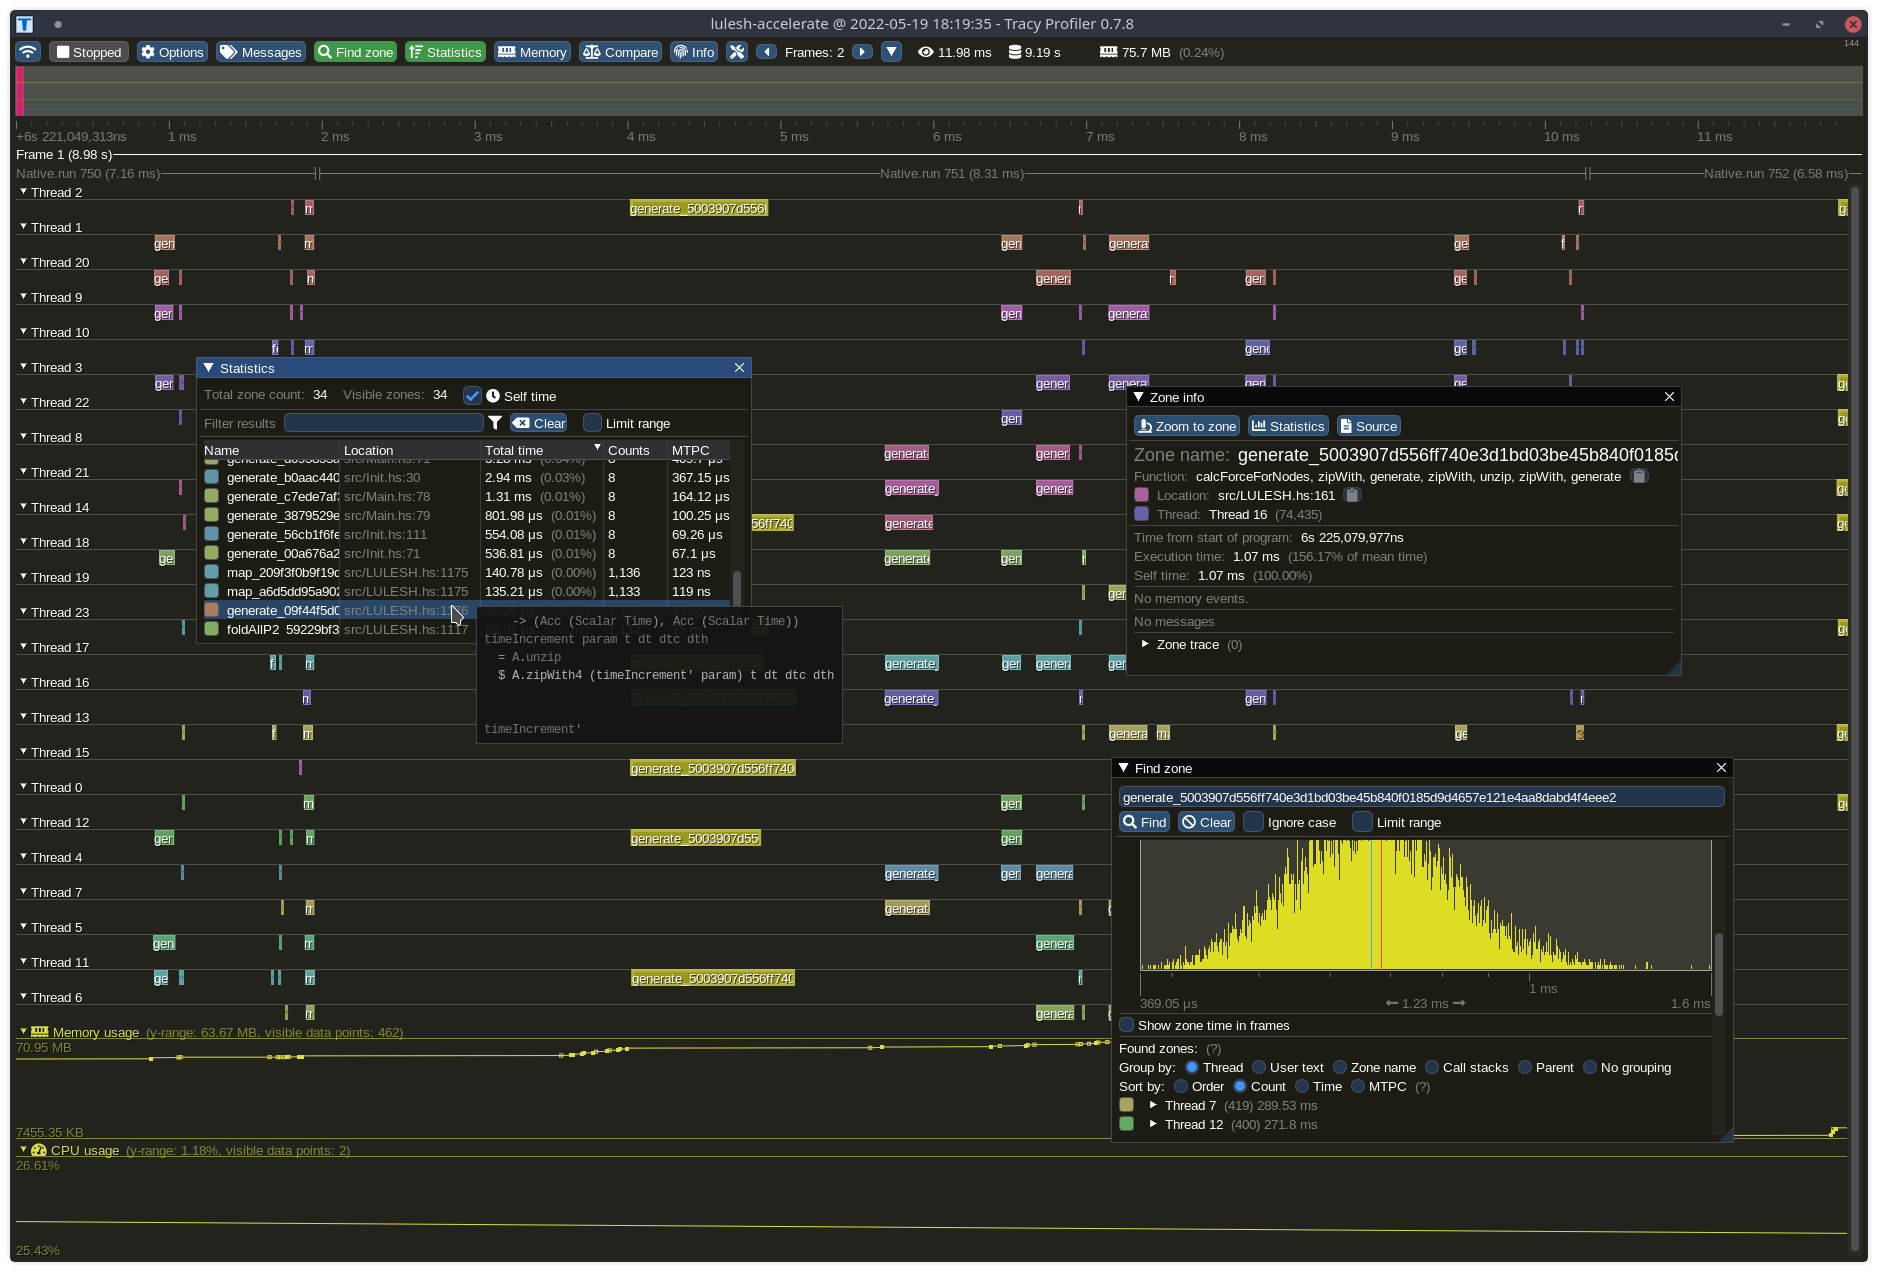
\includegraphics[width=\linewidth]{assets/tracy-lulesh-annotated.png}
  \caption{The LULESH-Accelerate~\cite{lulesh-accelerate} application running under the Tracy frame profiler. This screenshot demonstrates the additional context information made possible through the new annotation system.}\label{fig:tracy-lulesh-annotated}
\end{figure}

Figure~\ref{fig:tracy-lulesh-annotated} shows the result of running the
LULESH-Accelerate~\cite{lulesh-accelerate} application under Tracy with the
annotation system in place. This is a port of the LULESH~\cite{karlin2013lulesh}
mini-application, which is a highly simplified hydrodynamics simulation. Tracy's
output shows several \texttt{Native.run} calls along the horizontal axis. These
correspond to a single call of the iterative algorithm. The vertical lanes show
which computation kernels are being executed by each of the CPU's 24 threads at
a given time point, as well as the application's overall CPU usage and memory
consumption.

Previously, running this simulation under Tracy would also show these kernels
being executed, but without any context information beyond the automatically
generated kernel names. These are based on the kernel's main entry point
function and a hash of the optimized AST for that kernel. While this may not
pose any problems for simple programs, with more complex programs like this
LULESH implementation it can be difficult to tell which kernel belongs to which
part of the application as there is no direct link between them. However, with
the source mapping system in place the output now contains a lot more context
information that makes tracing the execution through the original program much
simpler. Notice how every kernel now shows file names and line numbers
corresponding to the location of the kernel's definition in the original source
code. Hovering over these locations now also opens a dialog showing an excerpt
from that source code. Also pay attention to the `\textsf{Function:}' field in
the zone info dialog. That field now shows the name stored in the top most stack
frame from the \emph{merged call stacks} discussed earlier. This is useful for
two reasons: first, it gives insight into how many array operations and more
specifically which array operations were fused into the kernel. The more
function names listed here, the better a job Accelerate's array fusion algorithm
did optimizing out unnecessary array operations. Secondly, this also shows the
explicit context information from Section~\ref{sec:explicit-context-information}
that was added to this part of the AST using a decorator function. Scattering
information like this throughout the program makes it simpler to get an at a
glance overview of what happens where in the program, and it also adds source
information to functions that might otherwise not have any due to limitations of
the source mapping system.

\subsubsection{Debug symbols}

% In this section I will talk about the ability to use the source mapping
% information to instrument the compiled program with (DWARF) debug symbols that
% can be used by a variety of already existing debuggers, profilers, and other
% tooling that doesn't need to have any specific knowledge of Accelerate to help
% diagnose problems with the compiled embedded programs. In the corrent
% implementation however the DWARF symbols that are part of the compiled binaries
% are picked up by tools like gdb and perf. I have not had the chance to look into
% fixing this due to a lack of time and an absence of documentation.

While specialized profiling tools like Tracy can be invaluable for getting
insight into the execution of a specific algorithm, their main weakness is that
they require the program to be manually instrumented with calls into an
accompanying profiling library. The more widespread approach to profiling and
debugging applications thus revolves around \emph{debug symbols} that are either
embedded in the application's binary or stored alongside it in an accompanying
metadata file. These debug symbols provide structural information about a region
of the program's binary that can be used to map back to parts of the original
program. This can range from descriptions of high level constructs like files,
namespaces, and subprograms, all the way down to function parameter
descriptions, jump labels, and individual expressions. The LLVM compiler's
metadata system is able to generate these debug symbols for a program by
annotating parts of the LLVM IR with special metadata tags. LLVM can then
generate debug information in a variety of supported formats, such as the
commonly used DWARF format~\cite{dwarf-debug-symbols}. Particularly interesting
for Accelerate is the ability to output debug information when targeting CUDA
through PTX.\@ Sadly, as of writing support for outputting debug information in
this format is incomplete. But if Accelerate already has full debug metadata
support by the time LLVM gets better support for this feature then Accelerate
should be able to benefit from better GPU debugging and profiling support using
NVIDIA's Nsight Systems without requiring any changes to Accelerate itself.
Because even though Nsight Systems does act like a frame profiler as mentioned
in the last section, it doesn't use explicit instrumentation like Tracy does and
instead relies on regular debug symbols.

The implementation of these debug symbols in Accelerate extends the backend with
several methods to annotate the LLVM IR AST with the aforementioned debug
information metadata. This is done by adding additional smart constructors to
the backend's internal deeply embedded IR language. These smart constructors can
generate local as well as global metadata definitions within the program.
Whenever Accelerate's LLVM CPU backend now creates a kernel function, the
backend also generates the associated debug metadata for that function. And when
LLVM compiles the IR, this metadata gets turned into DWARF debug symbols. In
theory this should be sufficient for sampling profilers like
\emph{perf}~\cite{perf-profiler-wiki} or debuggers like
\emph{gdb}~\cite{Stallman:1989:GMGa} to get information about the current kernel
that's being executed at a given point in time. Sadly, the details on how to
implement DWARF debug symbol support in LLVM are sparsely documented, and
currently this feature does not always work correctly. Still, with more work it
should be possible to get debugging and profiling working with these DWARF-based
tools on the kernel-level. And since the expressions contained within a kernel
also have source mapping information attached to them, it would also be possible
to extend the implementation to be able to support full expression-level
stepping debugging.

\subsection{Optimization flags}

% In this section I will go over all of the optimization flags that have been
% implemented in Accelerate and any relevant details in their implementation. This
% has a lot of overlap with the code generation and sharing recovery sections so
% this section may need to be merged in with those in some way.

While the source mapping was the main focus for this thesis, the secondary goal
was to find other uses for the annotation system.
Section~\ref{sec:optimizations} explored the idea of adding decorators to a
deeply embedded language that would change the compiler's optimization behavior
either for a single expression, for a subtree of the program, or for an entire
compilation unit by storing that information inside the annotations. Most of the
listed optimizations have been implemented in Accelerate and its LLVM backends.
As most of these optimizations directly influence the way code is being
generated, most of the implementation work was done within Accelerate's LLVM
backends. The exception here is the forcibly inlining of variables, as explained
in more detail a couple sections ago. Before discussing the other optimizations,
there is one more important detail to the forcibly inlining of terms that has
not yet been discussed.

\subsubsection{Inlining}

\begin{figure}[t]
  \centering
  \def\svgwidth{\linewidth}
  \import{assets/}{sharing-fusion-example.pdf_tex}
  \caption{An array program written in the Accelerate data-parallel array
    language. The dotted boxes indicate a single pass over the data after fusion
    has taken place. In this example, the result of \hask{map (+ 1) xs} being
    shared prevents this group of operations from fusing into a single
    kernel.}\label{fig:sharing-fusion-example}
\end{figure}

As alluded to when first discussing the optimization, other than getting rid of
potentially expensive memory operations, forcing terms to be recomputed can have
another advantage within the context of Accelerate. One limitation of
Accelerate's current array fusion system is that it can only fuse an array
operation that produces an array into at most one other array operation. Because
of that, array programs that fuse well tend to have a funnel-like structure
where produced arrays are either used to produce one array, or the array is
combined with other arrays to produce a single array. That in turn means that
when an output array is used as the input for two other array computations, then
array fusion is not possible with Accelerate's current fusion model. An example
of a situation where this is a problem is shown in
Figure~\ref{fig:sharing-fusion-example}. Here there is an input array called
\hask{xs} that has each of elements incremented by one. That incremented version
is then used in two other mapping operations, which are then summed together to
produce a result. With Accelerate's current array fusion model the bottom three
array operations that are surrounded by the dotted box can be fused together,
while the simple \hask{map (+1)} operation at the top of the figure needs to be
fully computed and written to memory before the fused kernel can be executed.
This is wasteful, as the time it takes to read and write this memory as well as
the time it takes to synchronize all participating threads within Accelerate's
scheduler greatly exceeds the time it would take to perform a single addition.
By simply changing that expression to \hask{forceInline (map (+1) xs)}, the
addition is now instead calculated as part of the two \hask{imap} calls, which
in turn allows the entire calculation from the figure to be fused into a single
operation.

\subsubsection{Loop unrolling}

The second optimization that has been implemented is the unrolling of loops. As
Accelerate's LLVM backends use an internal deeply embedded language for
constructing LLVM IR, these implementation is localized to two primitive loop
operations. The first operation iterates over an array with optional indices and
a certain step size, while the second operation accumulates a value as part of
the loop. Most other loop-based constructs supported by the backend are
implemented in terms of one of these two functions. And because the annotation
data for the current expression that is being converted to LLVM IR code was
already made accessible through an implicit parameter, implementing this did not
require any changes outside of these two functions. As a result, it would be
possible to implement similar optimization flags for performing other
algorithmic optimizations in the future with minimal unrelated code changes.
While the unrolling works as expected, one limitation of the current loop
unrolling implementation is that it will apply to all loops produced by an AST
node. Annotating a simple mapping function with \hask{unrollIters 16} will cause
the loop to be unrolled into chunks of sixteen elements as one might expect, but
doing the same thing with a two dimensional stencil operation will cause both
the inner and the outer loop to be unrolled. Coming up with a flexible method to
have more control over the unrolling behavior of nested and compound loop
operations would be an interesting subject for future research.

It is also worth noting that LLVM by itself already supports many common loop
transformations~\cite{llvm-code-transformation-metadata}. By simply adding
metadata annotations to the LLVM IR source code, LLVM's compiler should be able
to automatically perform those transformations to any program. Sadly, as of
writing the loop unrolling annotations don't do anything. And Clang, one of the
most prominent compilers for the C family of programming languages and the main
consumer of LLVM, also doesn't use this metadata. Still, when this does start to
work in a future revision of LLVM, then using this metadata to do the
optimizations instead of implementing them by hand before generating the IR
would both open up new optimization possibilities while simultaneously removing
complexity from Accelerate's LLVM backend.

\subsubsection{Other optimizations}

The last two optimization flags that were implemented are support for
controlling the \texttt{-ffast-math} behavior on a program subtree level, and
the ability to limit the number of registers that can be used by a thread in a
CUDA kernel. In the LLVM IR language, which \texttt{-ffast-math} semantics an
expression should use is set directly as an optional argument to the expression
itself. This makes it possible to allow these unsafe optimizations that don't
conform to the specifcation on specific operations, like a single addition and a
single multiplication, without affecting anything else. And because every
primitive scalar level expression in the annotated version of Accelerate's AST
contains an annotation, it is possible to map this idea one-to-one to Accelerate
programs. To recap, the idea is that the programmer can disable the
on-by-default \texttt{-ffast-math} behavior for an expression or an entire
kernel by decorating it with a \hask{withoutFastMath} combinator. It is also
possible to re-activate these optimizations for a smaller part of that
expression or kernel by using a similar \hask{withFastMath} decorator. During
sharing recovery these optimization flags are then written to the annotations
stored in all child nodes of the annotated subtree. As a result, when generating
LLVM IR code based on an expression, whether or not that expression should use
\texttt{-ffast-math} semantics can be queried by simply inspecting the current
expression's annotation that gets passed around using an implicit parameter.

The optimization flag for controlling the number of registers that may be used
by a CUDA kernel works by simply passing the value stored in the kernel's
annotations to the PTX assembler that turns PTX code into the GPU's equivalent
of machine code. While this is not particularly exciting, this way of using
annotations does open the door to other similar methods of programmatically
controlling compiler the compiler's overall behavior. One optimization flag that
has not yet been implemented but that would be very useful within the context of
Accelerate is the ability to control the architecture that kernels are compiled
for. Currently the CPU backend uses all of the instruction set features
available on the CPU that's compiled the program, and the CUDA backend uses the
latest architecture supported by the connected GPU.\@ Accelerate has an
interesting feature called \hask{runQ} that compiles the embedded program at
Haskell compile time and then embeds the binary for the compiled embedded
program into the compiled Haskell binary. When executing the host program, the
embedded program can then immediately run without needing to be compiled first.
With a couple of tweaks it would be possible to use the annotation system to
create kernels that target specific and even multiple architectures. Embedding
those into a compiled host program would make it possible to run the embedded
programs on a wider range of computers without requiring the full LLVM toolchain
to be installed on those computers.

\subsection{Results}

% Here I will talk about some of the benefits in terms of both performance and
% numerical stability offered by the annotation system as it is implemented in
% Accelerate. The other improvements in developer experience are difficult to
% quantify, although those have already been described in the previous sections on
% profiling and debugging. This section would list a couple of example programs
% that behave noticeably different when using the various optimization flags.
% Examples of these programs include:

% \begin{itemize}
%   \item The compensated summation algorithms. These don't produce the correct
%         results when using the on-by-default \texttt{-ffast-math} flags.
%         Disabling \texttt{-ffast-math} also greatly improves the numerical
%         stability of the saltmarsh simulation, but I do not think I can
%         reference that simulation here.
%   \item Programs that cannot fuse because an intermediate term is used as part
%         of two array operations. Inlining that term could allow the entire
%         program to be fused into a single operation. I would need to look it up,
%         but I remember an example using \hask{stencil2} where this exact thing
%         happened.
%   \item Some program where unrolling a loop increases the throughput.
%   \item A program that performs slightly better on the PTX backend when limiting
%         the number of registers to a power of two. The LULESH program can
%         benefit from this on certain GPUs, but I do not yet know if the
%         difference in performance is significant enough to be able to use it as
%         an example.
% \end{itemize}

% It would also be nice to talk about some of the other challenges I ran into
% surrounding GHC, LLVM, and the library and tooling ecosystem, but I don't think
% that fits anywhere here.

Previous sections already looked at what the addition of source information can
do for Accelerate programs in terms of improving the general development
experience. Now it is time to look at some of the more practical uses of having
access to the optimization flags from the previous section. As part of the
optimization process, Tracy is used to find the hotspots and to analyze how well
Accelerate is able to fuse array operations.

\subsubsection{Compensated summation}

The first example we will take a look at was the direct motivation for
implementing expression level \texttt{-ffast-math} configuration in Accelerate.
Computers usually store decimal numbers in a floating point format. With a
couple exceptions for special values and numbers that are too small to be
represented this way, this comes down to storing a number in the form of
$s \cdot m \cdot 2^{e}$, where $s$ indicates the sign with either a $-1$ or a
$1$ value, $m$ is a number in the half-open range $[1, 2)$, and $e$ is a
negative or positive exponent. This allows a wide ranger for numbers to be
represented even with a limited number of bits assigned to $m$ and $e$. But
because $m$ spans the $[1, 2)$ range with only a finite number of bits, not
every value between one and two can be represented. The difference between the
expected result of a floating point addition or multiplication and the value
stored by the computer is called the \emph{roundoff error}. This is the result
of the actual value being quantized to the closest matching value that can be
represented using $s$, $m$, and $e$. While in most cases these roundoff errors
tend to be so small that they can be safely ignored without causing any harm,
there are numerous situations where the accumulated roundoff errors from
repeated floating point operations add up to an amount that is actually
significant. As an example, the numbers $0.1$, $100.0$ and $1000.0$ can all be
perfectly represented by both single and double precision IEE-754 floating point
numbers, which is the floating point format used by all current consumer CPUs.
However, starting with a value of $0.0$ and then adding $0.1$ a thousand times
to that in a loop results in a total value of $99.99905$ for single and
$99.9999999999986$ for double precision rather than the expected value of
$100.0$. A similar situation occurs when summing very large or very small
floating point numbers. The four single-precision floating point numbers $1.0$,
$1.0$, $2.0^{100}$ and $-2.0^{100}$ should sum to $2.0$. But depending on the
order of the numbers, adding them up results in a value of either $0.0$ or
$1.0$, even though all of these numbers as well as the expected result can be
perfectly represented by a single precision floating point number. Because of
these reasons, people have come up with algorithms that try to compensate for
these rounding errors. This class of algorithms is aptfully named
\emph{compensated summation}~\cite{klein2006generalized}.

The \texttt{accelerate-blas} package implements several of these compensated
summation algorithms for
Accelerate~\footnote{\url{https://web.archive.org/web/20220523154459/https://github.com/tmcdonell/accelerate-blas/blob/master/src/Data/Array/Accelerate/Numeric/Sum.hs}}.
These algorithms keep track of the accumulated error from previous additions and
then compensate for that error in the next addition. While the exact details on
how this works are not important, it is relevant to understand that for this to
work, these algorithms need to perform additions and subtractions in a specific
order to be able to compute the error. However, as previously noted, for
performance reasons Accelerate always enables all of LLVM's unsafe floating
point math optimizations. And as a result, the compiler ends up reordering the
aforementioned additions and subtractions, breaking the compensated summation
algorithms. As a workaround, the \texttt{accelerate-blas} package currently
directly imports LLVM's addition and subtraction intrinsics through the foreign
function interface and uses those in place of Accelerate's regular addition and
subtraction operators. Doing so requires deep knowledge of Accelerate's
internals and the implementation also needs to be modified to use these new FFI
function calls. With the new annotation based optimization flags however, the
original unmodified version of the algorithm works as expected when wrapping it
with the \hask{withoutFastMath} decorator.

\subsubsection{LULESH}

Now it is time to take a look at how trivial usage of the loop unrolling
decorators affects the performance of the aforementioned Accelerate
implementation of the LULESH~\cite{karlin2013lulesh} hydrodynamics simulation.
More specifically, this section goes through the basic workflow of optimizing a
program based on profiling data. For brevity's sake the rest of this section
will link to specific lines in the LULESH implementation rather than citing them
directly.

\begin{figure}[t]
  \centering
  \def\svgwidth{\linewidth}
  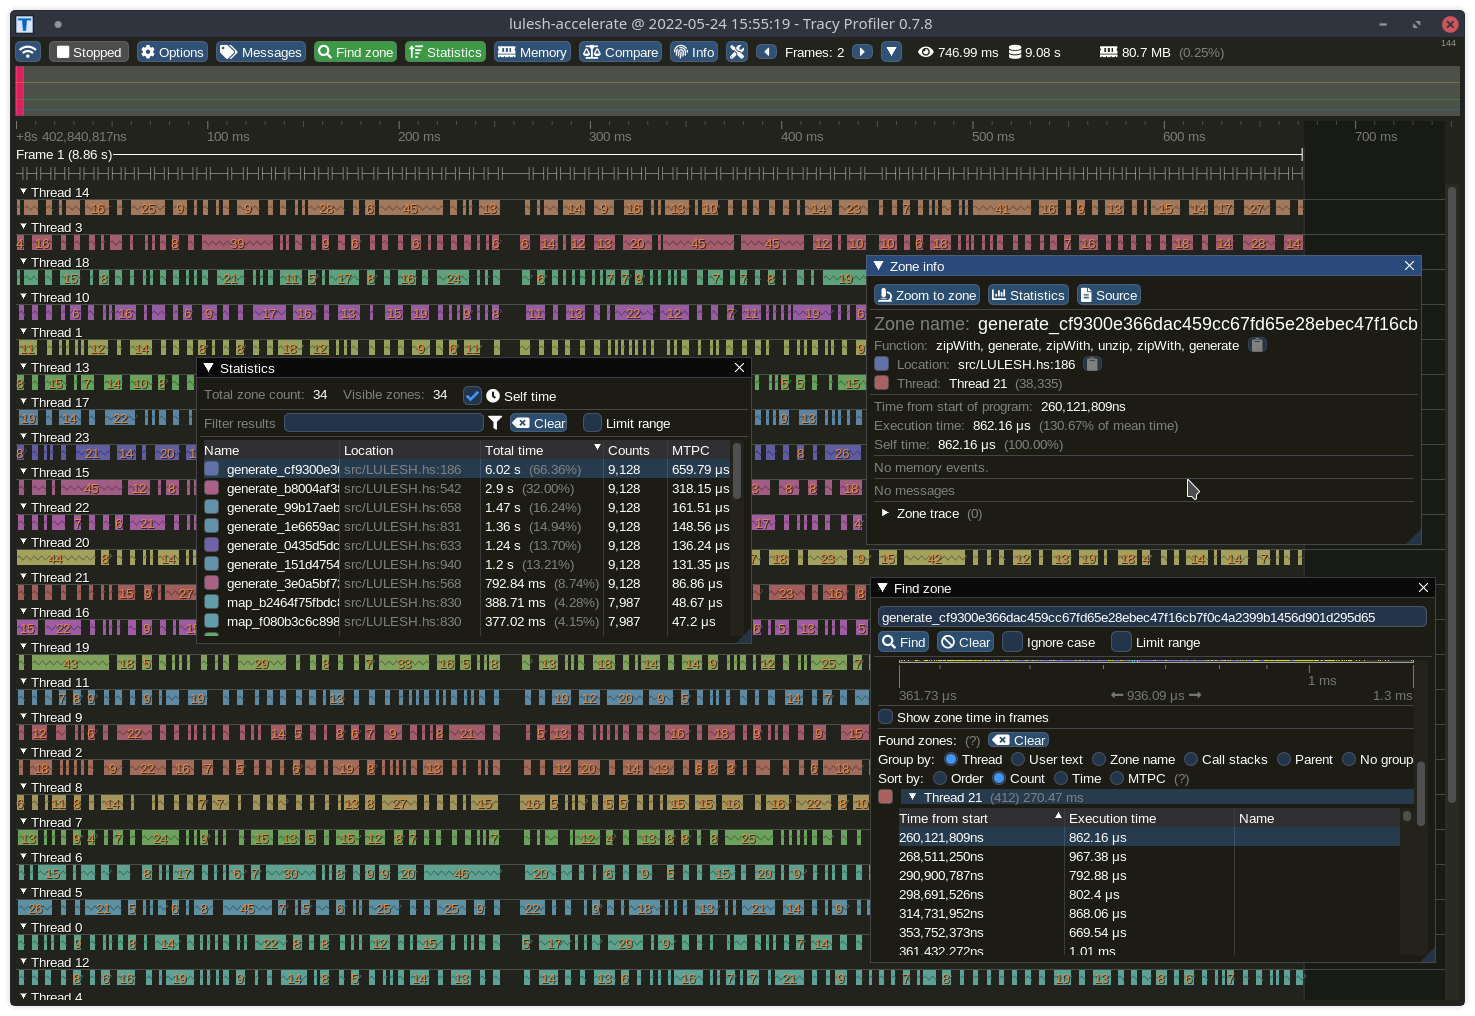
\includegraphics[width=\linewidth]{assets/tracy-lulesh-hotspots.png}
  \caption{Tracy showing hotspots in the LULESH-Accelerate~\cite{lulesh-accelerate} application. The highlighted \hask{generate} kernel been fused with five other operations.}\label{fig:tracy-lulesh-hotspots}
\end{figure}

The first step when optimizing any application is to find where the hotspots
are. Luckily, thanks to the new annotation system, Tracy was able to tell us
exactly where most of the time was being spent. A screenshot of Tracy's output
is shown in Figure~\ref{fig:tracy-lulesh-hotspots}. Over $65\%$ of an average
run's time is spent in the function that calculates forces for each element in
the
simulation\footnote{\url{https://github.com/robbert-vdh/lulesh-accelerate/blob/2618ebf7881d00a2052b9c4aee78c47c985484bb/src/LULESH.hs\#L165-L215}}.
This function shows up in Tracy as \texttt{zipWith, generate, zipWith, unzip,
  zipWith, generate}. That indicates to us that the compiler has been able to
fuse six different collective array operations into a single operation. Since
this is a hot loop, it may seem like a good candidate for manual unrolling.

Before making any changes, the unmodified program takes an average of $8.65$
seconds to run on an AMD Ryzen 9 5900x 12 core processor with SMT with a
standard deviation of $0.12$ seconds over the coarse of 30 runs. We'll prepend
\hask{unrollIters 8} to one of the Accelerate function calls in the function
linked above and\dots{}the runtime increased to an average wall runtime of
$9.60$ seconds with a standard deviation of $0.07$ seconds also over 30 runs.
What happened? As briefly discussed when first mentioning loop unrolling in
Section~\ref{sec:optimizations}, one potential drawback of loop unrolling is
that the number of times the loop is unrolled also causes the amount of
generated code to be multiplied by that amount, plus one more time for the tail
loop. As a potential consequence, the CPU may not be able to fit the entire loop
in its level-1 instruction caches anymore and it thus may need to fetch it from
either lower cache levels or from main memory. Running both the regular and the
eight times unrolled versions of the program under the Cachegrind tool that's
part of the Valgrind~\cite{nethercote2007valgrind} dynamic binary analysis
framework confirms this. Cachegrind is a tool that can precisely indicate what
the CPU's caches and branch predictor are doing at the instruction or source
line level by simulating those parts of the CPU.\@ Because Cachegrind needs to
simulate parts of a CPU, programs tend to run 20 to 100 times slower under
Cachgrind than they normally would. In the case of the LULESH application,
granular analysis is not needed a general overview of the program's overal cache
usage is sufficient to get the idea. Running both versions of the program under
Cachegrind for one minute shows very different cache usage statistics. As
expected, the data cache usage for both versions is almost identical, but the
instruction cache miss rate increases from $0.30\%$ to $4.18\%$ for the first
level instruction caches and from $0.01\%$ to $0.07\%$ for the last level
instruction caches when comparing the original and the unrolled versions. And to
make matters worse, these numbers also include the identical shared setup phase
of the program that takes up the first 20 seconds of the 60 seconds spent
profiling. It is thus no surprise that the unrolled version is slower.

However, things change when switching over to Accelerate's GPU backend. When
running both the original program and the eight times unrolled version on an
NVIDIA RTX 2080 SUPER GPU, the unrolled version now ends up being significantly
faster. With that GPU the average runtimes and standard deviations over 30 runs
are $3.13$ and $0.04$ seconds for the original version, with $3.07$ and $0.04$
for the unrolled version. While this is only a $1.8\%$ speedup, it is free
performance that only required a tiny change to the code. With different
unrolling amounts the speedup may be smaller or larger and the specific GPU used
also plays a role, so optimizing a program like this still involves some degree
of experimentation. The reason why only eight times unrolling was tested here is
because both the CPU and GPU versions of the embedded LULESH program are
compiled at Haskell compile time, and Accelerate's LLVM backends currently does
not handle large amounts of LLVM IR well. Particularly on the CPU backend
unrolling more than a couple times would increase compile times exponentially.
So to make the comparison fairer, the same settings were tested for both
backends.

\section{Discussion and future work}

Having an annotation system for a language like Accelerate opens up the door for
both better development experiences and more opportunities to hand optimize
embedded programs. The current implementation enables new profiling based
optimization workflows whereas previously this process would mostly be driven by
trial and error. But more importantly, it also forms a framework that can be
built upon. Right now the captured source information is only used to add
kernel-level context information for the Tracy frame profiler, but the optimized
ASTs contain line-level source locations that can be used to enable step
debugging and give more detailed insights into the runtime of a program.
Similarly, the optimization options backed by the annotation system mostly serve
as a proof of concept. For instance, the loop unrolling optimization could be
turned into a more general loop optimization construct that would allow the
programmer to better finetune Accelerate's multidimensional, sequential and
fused loops.

Another aspect that has not yet been explored in the context of deeply embedded
languages is using the annotation and source location systems to improve the
experience of the language's compilation process. Source locations can be used
to provide detailed warnings during compilation, for instance when the compiler
wants to fuse together array operations with incompatible optimization flags or
when detecting common mistakes. These warnings can also be suppressed by
introducing new annotation based decorators. Aside from diagnostics, annotations
could also be used to generate multiple variants of an embedded program that are
optimized to run on different target processor features in order to increase the
portability of a compiled embedded program that has been embedded inside of an
executable binary. In conclusion, the annotation system enables new workflows
while also forming the foundations for a new area of exploration.

\appendix
\section{Source code}\label{sec:source-code}

The implementation for the annotation system as implemented in Accelerate can be
found in the GitHub repositories for the forked
\texttt{accelerate}\footnote{\url{https://github.com/robbert-vdh/accelerate/tree/feature/force-inline}}
and the
\texttt{accelerate-llvm}\footnote{\url{https://github.com/robbert-vdh/accelerate-llvm/tree/feature/tracy-annotations}}
packages. The
\hask{Data.Array.Accelerate.Annotations}\footnote{\url{https://github.com/robbert-vdh/accelerate/blob/feature/force-inline/src/Data/Array/Accelerate/Annotations.hs}}
module in the \texttt{accelerate} fork contains a complete guide on how to
migrate Accelerate libraries to the new annotated version of Accelerate. Take a
look at the
\texttt{linear-accelerate}\footnote{\url{https://github.com/robbert-vdh/linear-accelerate/tree/feature/annotations}}
fork for an example on how to do this.

\printbibliography{}

\end{document}
